\documentclass[11pt]{article}

\usepackage[margin=1in]{geometry}
\usepackage[T1]{fontenc}
\usepackage{amsmath}
\usepackage{array}
\usepackage{booktabs}
\usepackage{caption}
\usepackage{graphicx}
\usepackage{indentfirst}
\usepackage[protrusion=true,expansion=false]{microtype}
\usepackage{placeins}
\usepackage[numbers]{natbib}
\usepackage{hyperref}

\graphicspath{{../figures/}}
\setlength{\parindent}{1.5em}
\setlength{\parskip}{0pt}
\captionsetup{font=small,labelfont=bf}
\newcommand{\paperfigwidth}{0.80\linewidth}

\title{BEACON: Bayesian Event Assessment for Conjunction Observation and Notification}
\author{Zander Polk}
\date{\today}

\begin{document}
\maketitle

\begin{abstract}
Satellite conjunction assessment is a rare-event decision-support problem in which operators must prioritize a small number of potentially high-risk events from a much larger set of routine conjunction warnings. This work introduces BEACON, a reproducible study of calibrated, uncertainty-aware machine learning for satellite conjunction triage using public conjunction data message data.

BEACON evaluates event-level risk prediction across early, 3-day, 2-day, and 1-day warning horizons using leakage-safe event splits. The study compares learned models against a direct current-risk baseline, evaluates probability calibration, tests whether bootstrap ensemble uncertainty can identify events that should be escalated for human review, and ablates the CDM-provided current risk feature.

Across 20 repeated event-level train/validation/test splits, learned gradient boosting models improve rare-event ranking over direct current-risk ranking at every evaluated horizon. The strongest repeated-split PR-AUC values are 0.806 at 1 day, 0.630 at 2 days, 0.493 at 3 days, and 0.233 at the early horizon, compared with current-risk baseline PR-AUC values of 0.581, 0.367, 0.237, and 0.109 respectively. A current-risk feature ablation shows that removing the current risk feature reduces gradient-boosting PR-AUC at every horizon, but the no-risk model still exceeds direct current-risk PR-AUC. At the 10\% escalation level, bootstrap uncertainty captures 97.5\% of high-risk events at 1 day, 96.3\% at 2 days, 97.5\% at 3 days, and 80.8\% at the early horizon, far above random escalation. Current-risk escalation remains a very strong comparator, so uncertainty is best interpreted as a complementary human-review signal rather than a replacement for domain risk estimates.
\end{abstract}

\section{Introduction}

Satellite operators face an increasingly congested orbital environment. Collision avoidance decisions are high-consequence, time-sensitive, and uncertainty-heavy. Because truly high-risk conjunctions are rare, the task is not simply classification. It is rare-event triage.

A useful decision-support system should do more than maximize accuracy. It should rank risky events effectively, produce probabilities that are reasonably calibrated, and communicate uncertainty so that ambiguous cases can be escalated for human review.

This project studies whether lightweight machine learning models can support conjunction assessment by improving rare-event risk ranking, probability calibration, uncertainty-aware escalation, robustness across repeated event-level splits, and transparent interpretation of how much performance depends on the current CDM risk estimate.

BEACON is not intended to replace operational conjunction assessment systems. It is a research prototype for evaluating how machine learning should be tested when applied to space-safety decision support.

\section{Research Questions}

\begin{description}
    \item[RQ1] Can lightweight machine learning models predict high-risk satellite conjunction events from public CDM data?
    \item[RQ2] How does performance change across early-warning horizons before closest approach?
    \item[RQ3] Do learned models improve rare-event ranking over direct current-risk ranking?
    \item[RQ4] Are predicted risk scores calibrated enough to support decision-making?
    \item[RQ5] Can uncertainty estimates identify predictions that should be escalated for human review?
    \item[RQ6] Are the main findings stable across repeated event-level train/validation/test splits?
    \item[RQ7] How much of the learned model's performance depends on the CDM-provided current risk feature?
\end{description}

\section{Related Work}

\subsection{Space debris, conjunction assessment, and collision avoidance}

Spacecraft collision avoidance is motivated by the long-term growth of orbital traffic and debris. Kessler and Cour-Palais's classic debris-cascade work showed that collisions in dense orbital regions can generate additional debris and increase future collision risk \citep{kessler1978collision}. Modern conjunction assessment workflows therefore require operators to monitor close approaches, estimate risk under uncertainty, and decide which events deserve additional analysis or mitigation.

BEACON does not attempt to model orbital dynamics directly or recommend avoidance maneuvers. Instead, it focuses on the machine-learning evaluation layer: given public conjunction data messages, can a model produce calibrated, uncertainty-aware triage signals while avoiding leakage and overclaiming?

\subsection{Machine learning for conjunction risk prediction}

The closest prior work is the ESA Spacecraft Collision Avoidance Challenge, which released a curated dataset of conjunction data messages and asked participants to predict final collision risk \citep{uriot2020spacecraft}. That work established the dataset, competition framing, and the usefulness of machine learning for studying collision-risk evolution.

BEACON builds on this direction but emphasizes a different set of research concerns. Rather than only asking whether a model can predict final risk, BEACON focuses on trustworthy evaluation: event-level splits, early-warning horizons, calibration, uncertainty-aware escalation, repeated split robustness, and current-risk feature ablation. This positions BEACON as a reproducible evaluation artifact rather than an operational collision-avoidance model.

\subsection{Probability calibration}

Calibration is central when model outputs may support decisions. The Brier score is a classic metric for evaluating probabilistic forecasts \citep{brier1950verification}. Platt scaling introduced a practical method for mapping classifier scores to calibrated probabilities \citep{platt1999probabilistic}, and later work showed that supervised models can differ substantially in probability quality even when their ranking performance is strong \citep{niculescu2005predicting}. Guo et al. demonstrated that high-performing modern neural networks can be poorly calibrated and that simple post-hoc calibration can be effective \citep{guo2017calibration}.

BEACON follows this line of work by treating probability quality as a separate evaluation target from ranking. It reports Brier score, Expected Calibration Error, reliability curves, and quantile-binned reliability curves, because rare-event probabilities are concentrated near zero and can be hard to interpret with ordinary linear bins.

\subsection{Uncertainty estimation and human review}

Bayesian and Bayesian-inspired methods are widely used to express model uncertainty. Gal and Ghahramani interpreted dropout as approximate Bayesian inference \citep{gal2016dropout}, while Kendall and Gal distinguished epistemic uncertainty from aleatoric uncertainty and argued that uncertainty estimates are important for decision-making in high-consequence prediction settings \citep{kendall2017uncertainties}.

BEACON includes a true Bayesian logistic regression baseline and a bootstrap gradient-boosting ensemble. The bootstrap ensemble is Bayesian-inspired rather than fully Bayesian, but it provides a practical predictive-disagreement signal. BEACON evaluates this uncertainty signal as a human-review escalation policy rather than as an automated decision rule.

\subsection{Rare-event evaluation}

Conjunction triage is highly imbalanced, with high-risk events forming a small fraction of the dataset. In such settings, accuracy can be misleading. Precision-recall analysis is often more informative than ROC analysis for imbalanced binary classification, because it focuses directly on performance for the rare positive class \citep{saito2015precision}.

BEACON therefore emphasizes PR-AUC, top-K precision and recall, and positive escalation rate. These metrics match the operational framing better than accuracy: the practical question is whether a limited review budget can capture the small number of events most likely to matter.

\section{Data}

The dataset consists of public conjunction data messages grouped by event. Each event contains one or more CDM observations before time of closest approach.

The high-risk label is defined using the final available pre-TCA event risk. A conjunction is labeled high-risk if its final $\log_{10}$ risk is greater than or equal to $-5$, corresponding to a collision probability threshold of $10^{-5}$.

The resulting task is highly imbalanced. In the repeated test splits used here, the mean positive rate is 0.6079\%, corresponding to about 12 high-risk events per test horizon. This makes accuracy a poor evaluation metric. A model that predicts every event as non-high-risk would achieve very high accuracy while being operationally useless.

\section{Horizon Construction}

BEACON evaluates prediction snapshots at four warning horizons: early, 3d, 2d, and 1d. The early horizon is the earliest available CDM per event. The 3d, 2d, and 1d horizons use the closest available CDM at least 3, 2, and 1 days before TCA respectively.

A horizon coverage diagnostic is included because not every event contains observations at every requested warning horizon.

\begin{figure}[!htbp]
    \centering
    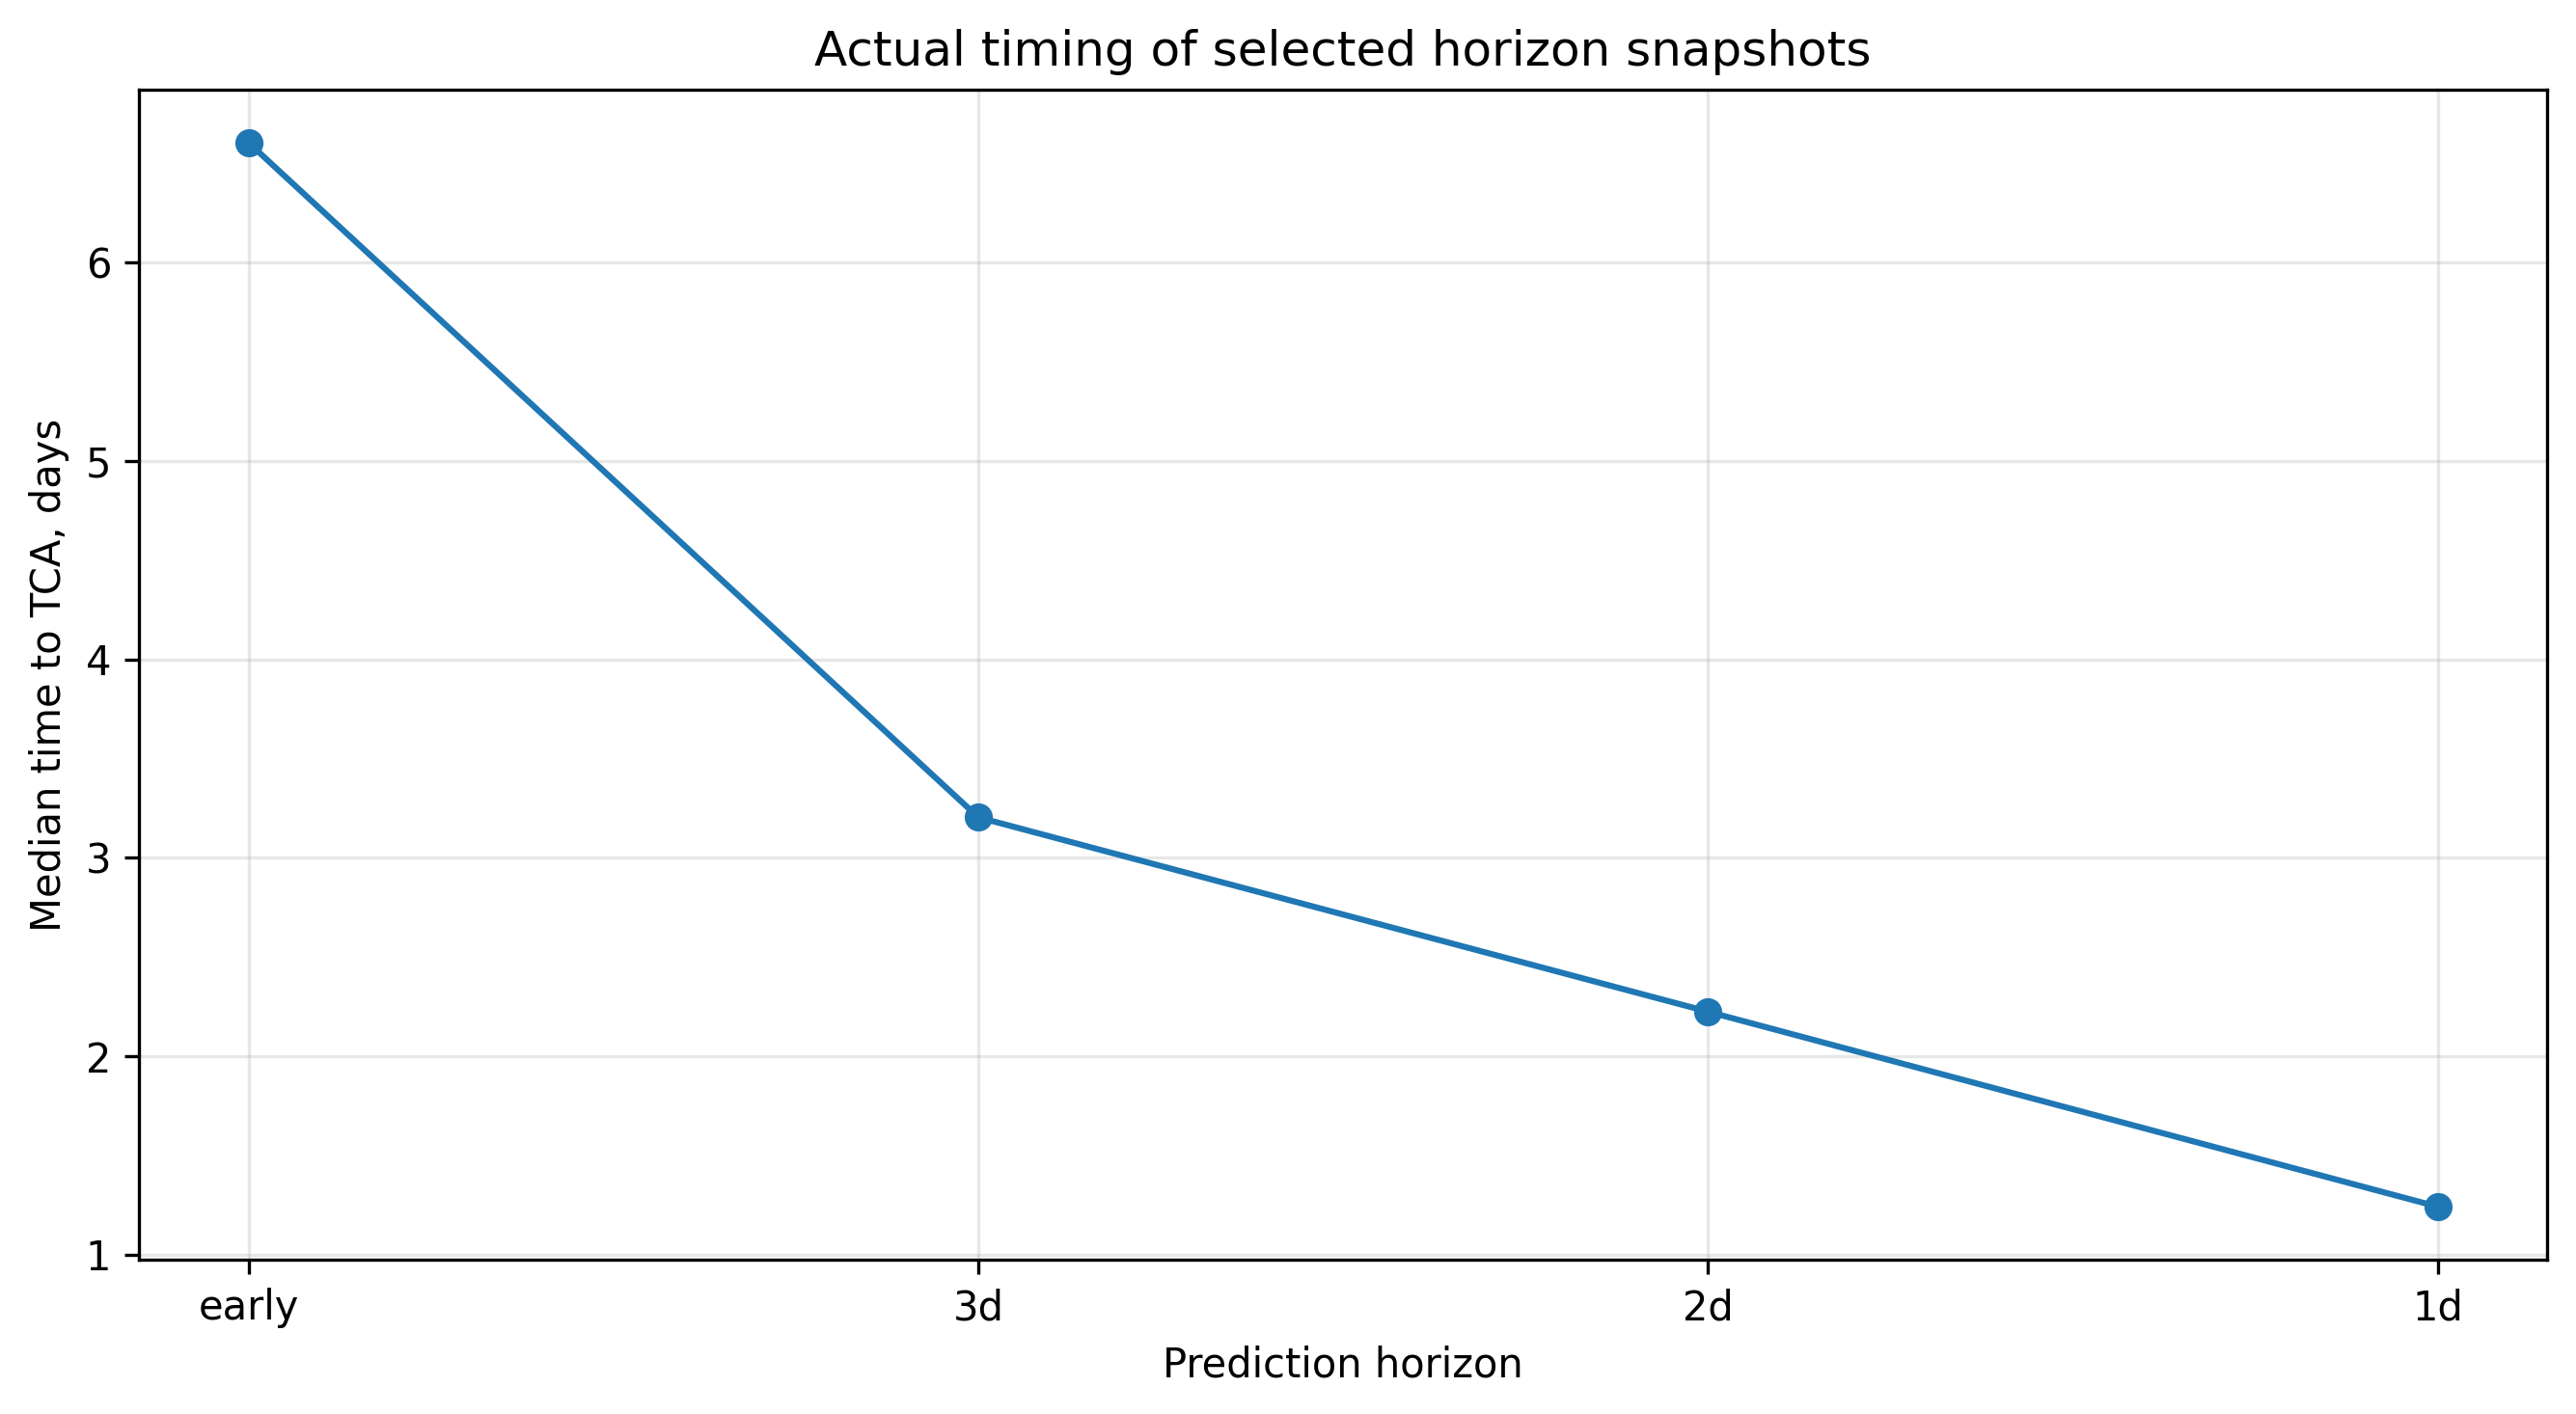
\includegraphics[width=\paperfigwidth]{horizon_timing.png}
    \caption{Actual timing of selected horizon snapshots.}
    \label{fig:horizon-timing}
\end{figure}

\begin{figure}[!htbp]
    \centering
    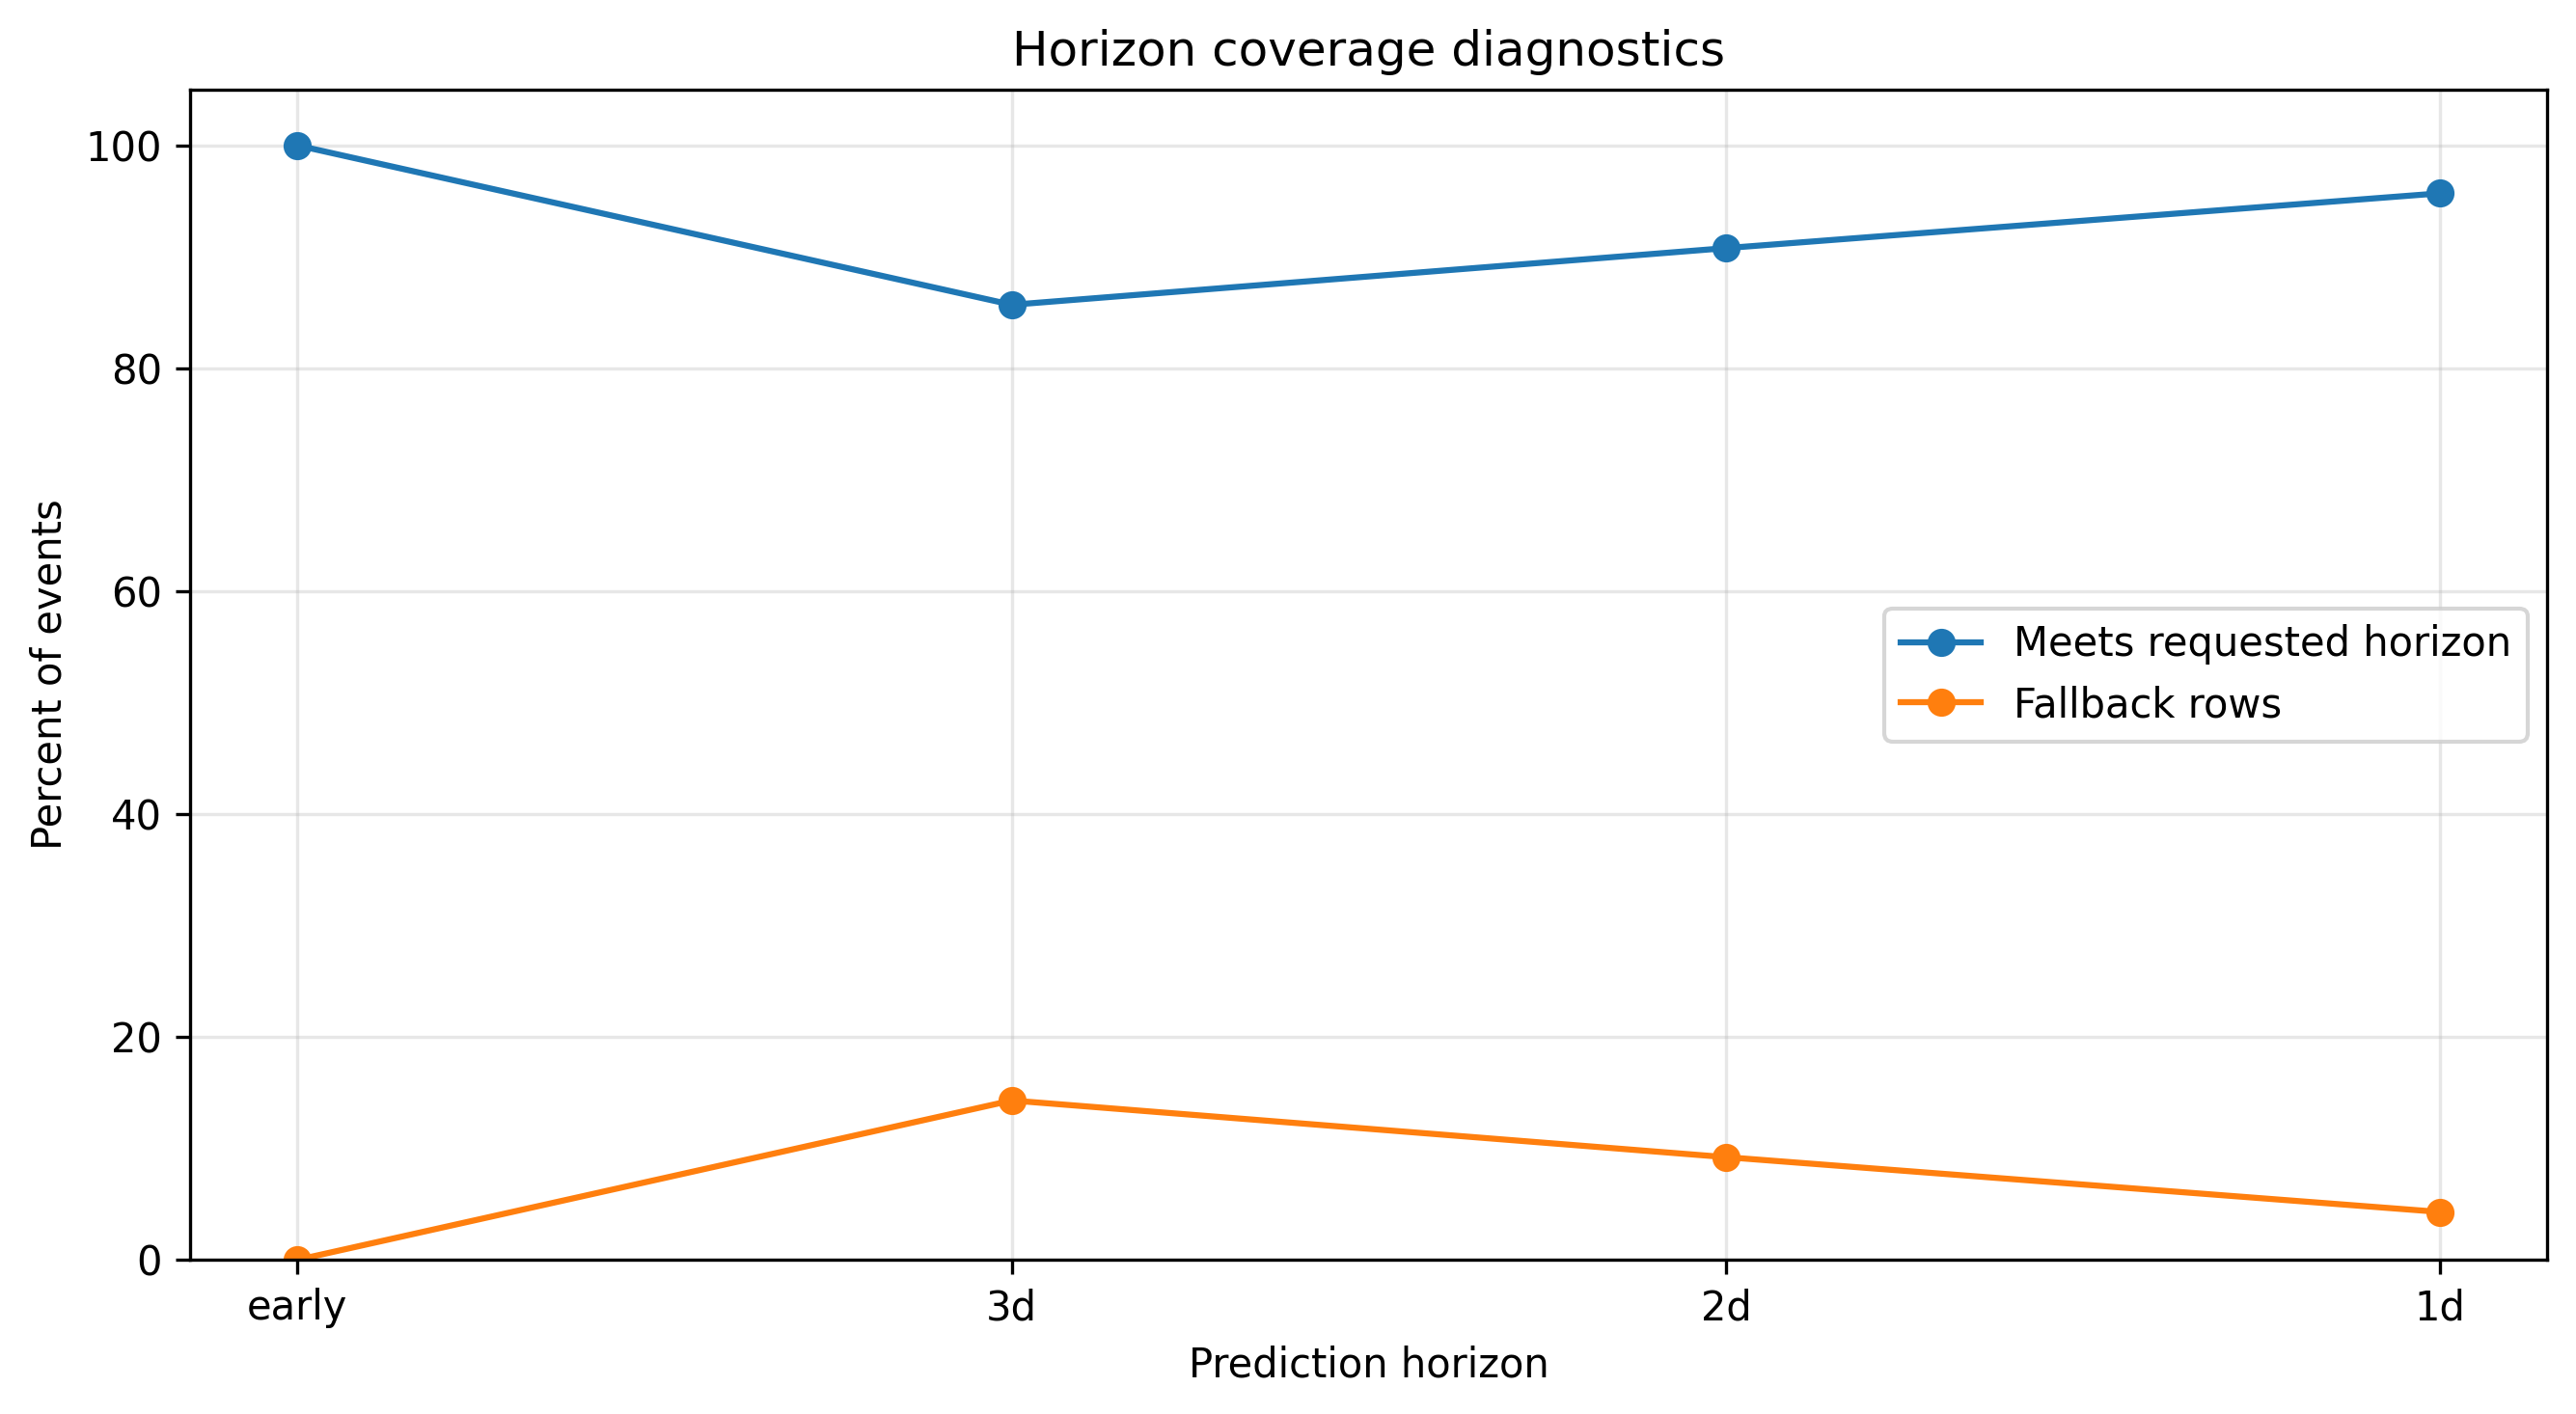
\includegraphics[width=\paperfigwidth]{horizon_coverage.png}
    \caption{Horizon coverage diagnostics.}
    \label{fig:horizon-coverage}
\end{figure}

The original plan included a 7-day horizon, but the dataset did not contain valid 7-day snapshots for the events in this split. Instead, BEACON reports an early horizon, defined as the earliest available CDM for each event. This is more honest than labeling the earliest available observations as true 7-day predictions.

Preprocessing prefers pre-TCA observations for all horizon snapshots and final label construction. If an event has no pre-TCA observations, the pipeline falls back to an available row and records the selected-row status in \texttt{results/horizon\_post\_tca\_diagnostics.csv}. This makes post-TCA fallback behavior explicit rather than silently mixing it into the results.

\FloatBarrier

\section{Methods}

\subsection{Event-level splitting}

Train, validation, and test splits are performed by \texttt{event\_id}, not by individual CDM row. This prevents observations from the same conjunction event from leaking across splits.

This design rule is critical because each event may have multiple CDM observations. If rows from the same event appeared in both training and test sets, the model could appear to perform well by recognizing event-specific information rather than learning generalizable risk structure.

\subsection{Baselines and learned models}

The study compares four baseline approaches: current-risk baseline, logistic regression, random forest, and gradient boosting.

The current-risk baseline ranks events directly by the CDM-provided current risk estimate. This is an important baseline because the existing risk value is already highly informative.

Learned models are allowed to use the current CDM risk feature along with the other numeric CDM/context features. Therefore, the intended comparison is not machine learning without risk versus current risk. The intended comparison is whether a learned model can improve triage over direct current-risk ranking by combining current risk with additional features.

Final-risk label metadata, including \texttt{final\_risk} and \texttt{final\_time\_to\_tca}, is excluded from model features to avoid label leakage.

\subsection{Current-risk feature ablation}

To make the role of the CDM risk feature explicit, BEACON includes a current-risk feature ablation. The ablation compares three policies across the same repeated event-level splits: direct current-risk ranking, gradient boosting with the current risk feature included, and gradient boosting with the current risk feature removed.

This experiment separates two claims. First, it tests whether a learned model can improve over simply sorting by the current risk estimate. Second, it tests whether non-risk CDM/context features contain useful signal when the current risk estimate is unavailable to the learned model.

\subsection{Calibration}

Gradient boosting probabilities are calibrated using sigmoid calibration on the validation split. Calibration is evaluated on held-out test events using Brier score, Expected Calibration Error, reliability curves, and quantile-binned reliability curves.

Calibration is important because a model can rank events well while still producing probabilities that are poorly aligned with observed event frequencies.

\subsection{Bayesian and Bayesian-inspired uncertainty estimation}

BEACON includes a Laplace-approximated Bayesian logistic regression baseline. This model uses a Gaussian prior, Bernoulli likelihood, MAP estimation, and a local Gaussian posterior approximation. It provides a true Bayesian probabilistic baseline, although it is not the strongest ranking model in the current experiments.

BEACON also uses a bootstrap gradient boosting ensemble as a Bayesian-inspired uncertainty estimator. Multiple gradient boosting models are trained on bootstrapped samples of the training data. For each event, BEACON computes the mean predicted probability across ensemble members and the predictive standard deviation across ensemble members.

The predictive standard deviation is used as an uncertainty score. Events with the highest uncertainty can be escalated for human review.

The bootstrap ensemble is called Bayesian-inspired rather than fully Bayesian because it does not explicitly define priors, likelihoods, or posterior inference over the gradient boosting model. Instead, it approximates uncertainty by measuring disagreement across models trained on plausible resampled versions of the data.

\subsection{Repeated split robustness}

Because high-risk conjunctions are rare, a single fixed test split can be sensitive to which high-risk events appear in the test set. To reduce this risk, BEACON repeats the event-level train/validation/test split across 20 random seeds and reports mean and standard deviation for ranking, calibration, top-K recall, escalation metrics, and risk ablation metrics.

This robustness check changes the interpretation of the results. Rather than relying on a single split, BEACON asks whether the main trends persist across many leakage-safe event-level splits.

\section{Metrics}

The primary metrics are ROC-AUC, PR-AUC, Brier score, Expected Calibration Error, precision at top 1\%, 5\%, and 10\%, recall at top 1\%, 5\%, and 10\%, positive escalation rate under uncertainty-based review, risk-ablation deltas, and repeated-split mean and standard deviation.

Accuracy is not emphasized because the positive class is extremely rare. For rare-event triage, the most important operational question is not whether the model predicts every event correctly. The more important question is whether it helps prioritize the small number of events most deserving of attention.

\section{Results}

\subsection{Rare-event ranking}

Across 20 repeated event-level splits, learned models improve PR-AUC over the current-risk baseline at every evaluated horizon.

\begin{table}[!htbp]
\centering
\caption{Repeated-split PR-AUC by horizon. Values are mean $\pm$ standard deviation across 20 event-level splits.}
\label{tab:ranking}
\begin{tabular}{llcc}
\toprule
Horizon & Best learned model & Best learned PR-AUC & Current-risk PR-AUC \\
\midrule
1d & Bootstrap gradient boosting ensemble & $0.806 \pm 0.091$ & $0.581 \pm 0.085$ \\
2d & Bootstrap gradient boosting ensemble & $0.630 \pm 0.106$ & $0.367 \pm 0.083$ \\
3d & Gradient boosting & $0.493 \pm 0.090$ & $0.237 \pm 0.048$ \\
Early & Gradient boosting & $0.233 \pm 0.082$ & $0.109 \pm 0.031$ \\
\bottomrule
\end{tabular}
\end{table}

\begin{figure}[!htbp]
    \centering
    \includegraphics[width=\paperfigwidth]{repeated_split_pr_auc.png}
    \caption{Repeated split PR-AUC robustness.}
    \label{fig:repeated-pr-auc}
\end{figure}

\begin{figure}[!htbp]
    \centering
    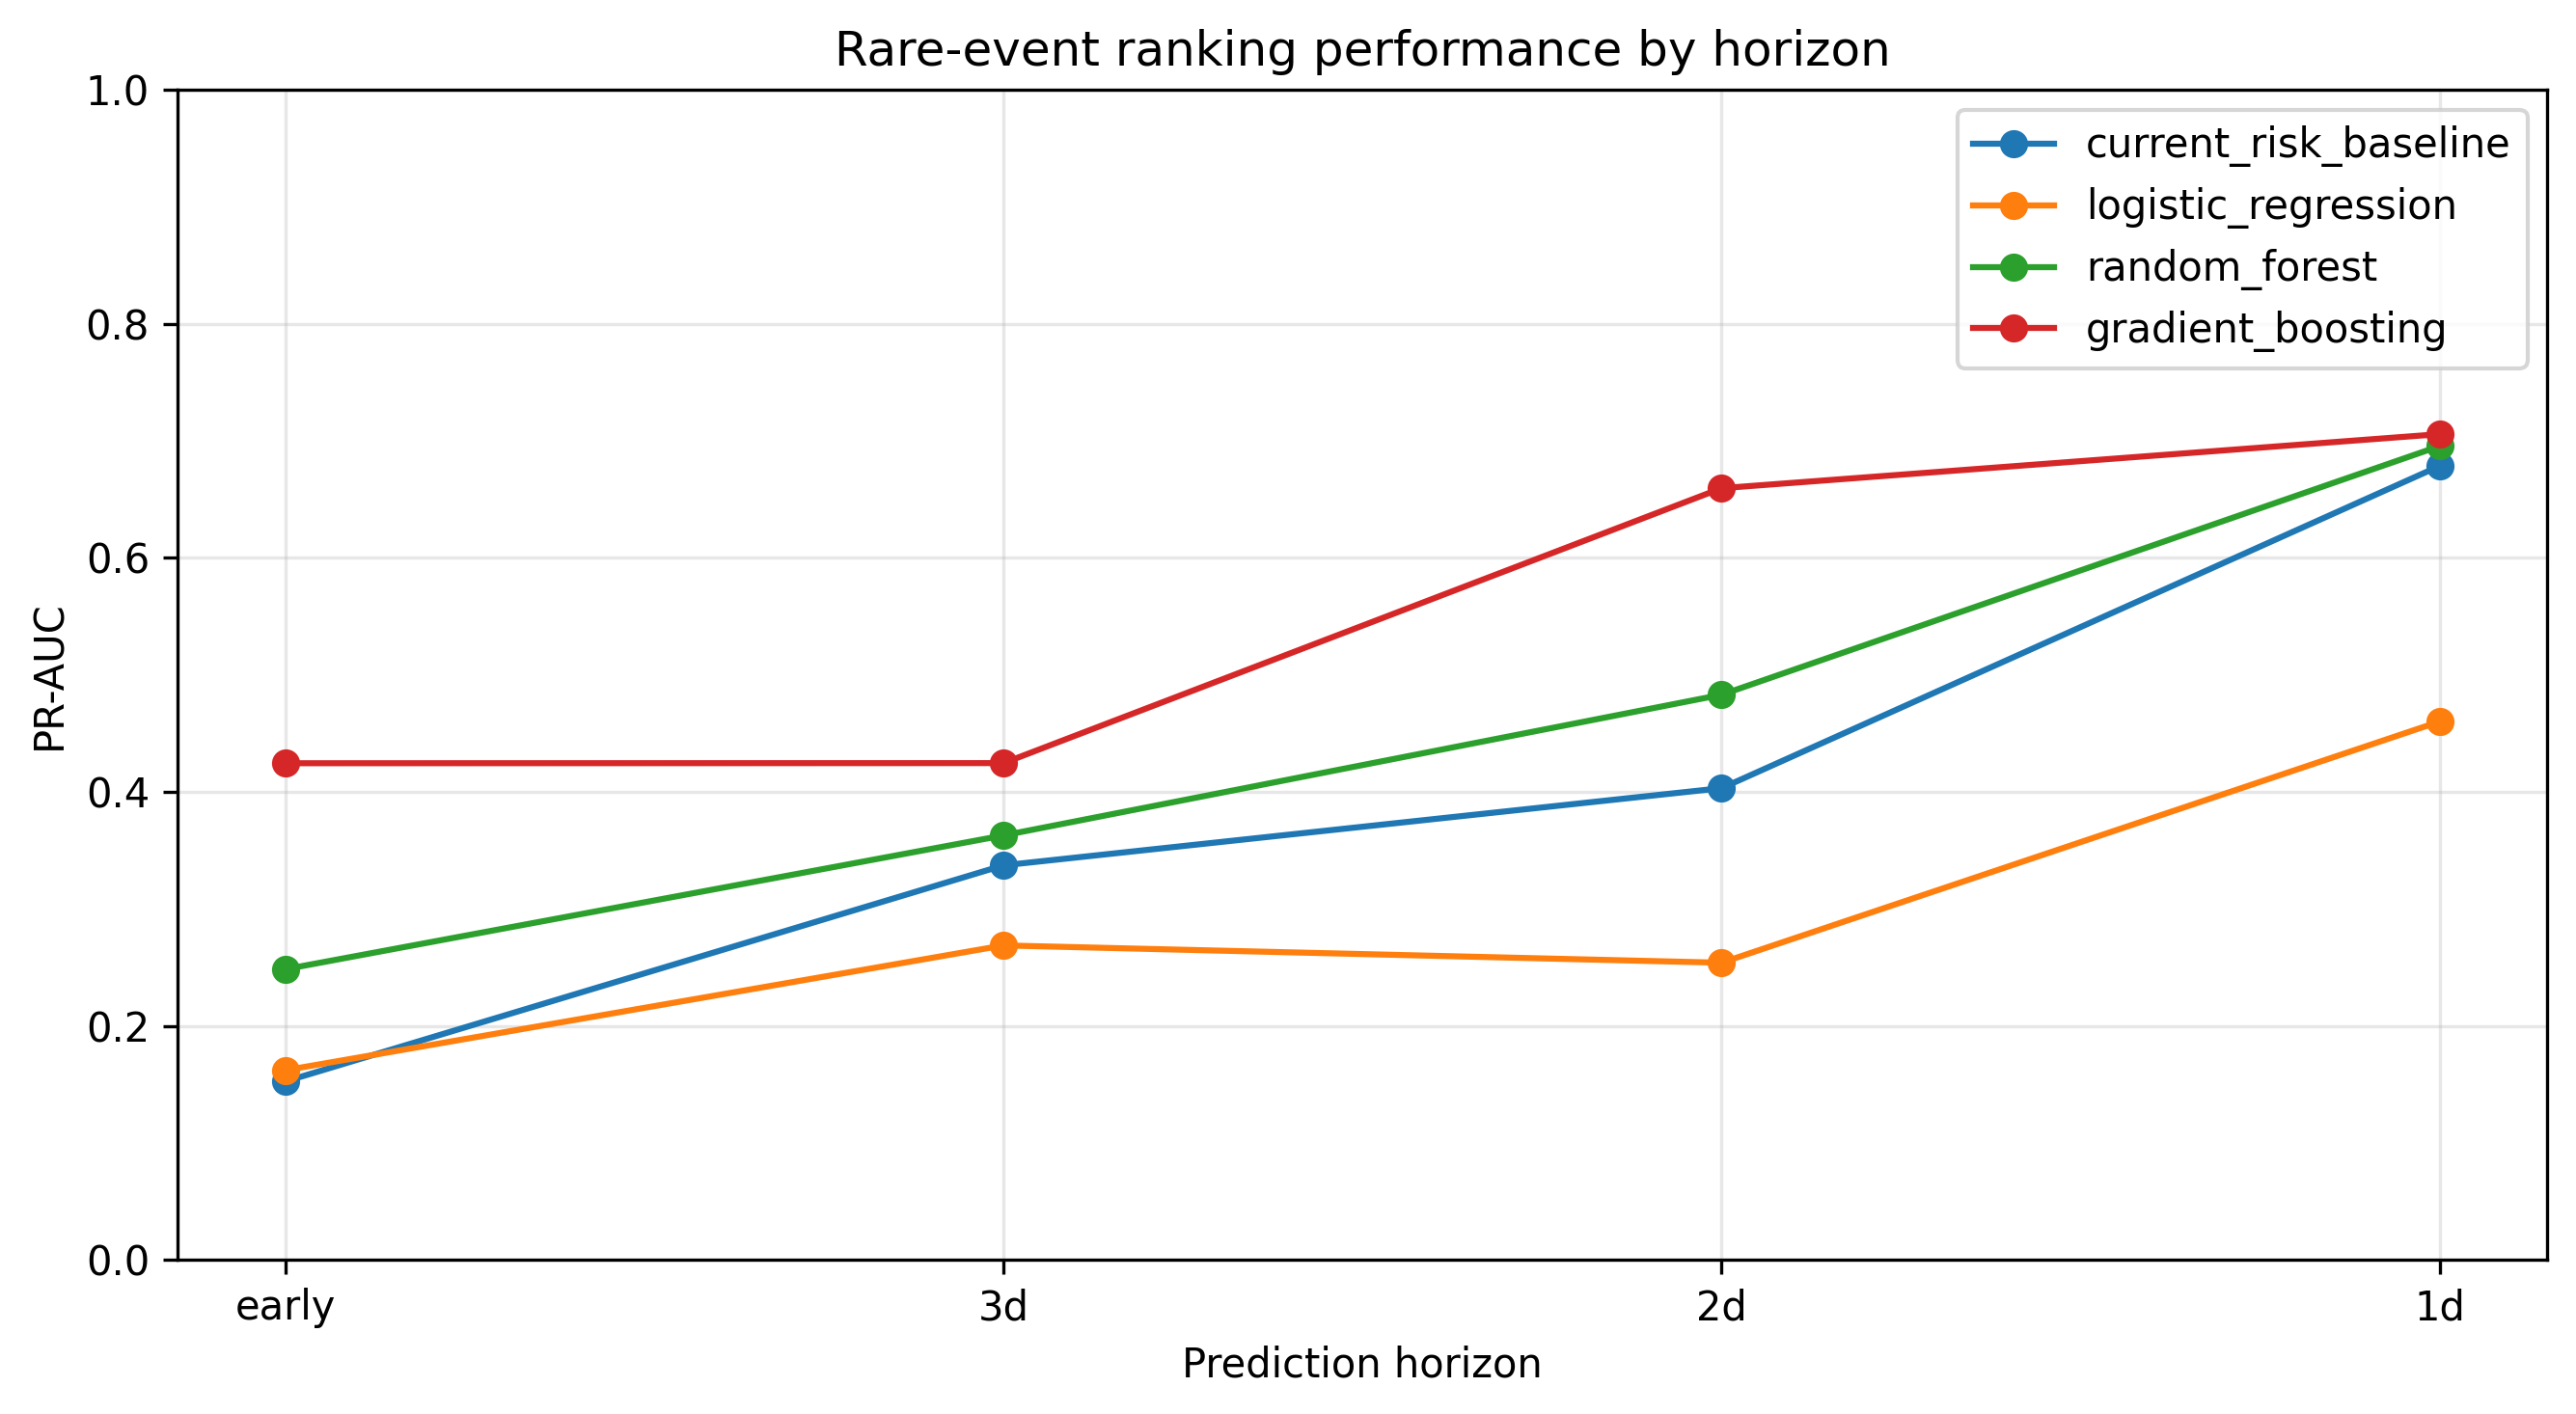
\includegraphics[width=\paperfigwidth]{pr_auc_by_horizon.png}
    \caption{PR-AUC by prediction horizon.}
    \label{fig:pr-auc-horizon}
\end{figure}

The current-risk baseline remains strong, which is expected. The CDM risk estimate is already a meaningful domain signal. However, the repeated split results show that learned models add ranking value beyond direct current-risk ranking, especially at 1-day, 2-day, and 3-day horizons.

\FloatBarrier

\subsection{Top-K triage}

Top-K recall measures how many high-risk events are captured when reviewing only the highest-ranked events. This is especially relevant for operational triage, where human attention is limited.

\begin{figure}[!htbp]
    \centering
    \includegraphics[width=\paperfigwidth]{repeated_split_top5_recall.png}
    \caption{Repeated split top-5\% recall robustness.}
    \label{fig:top5-robustness}
\end{figure}

\begin{figure}[!htbp]
    \centering
    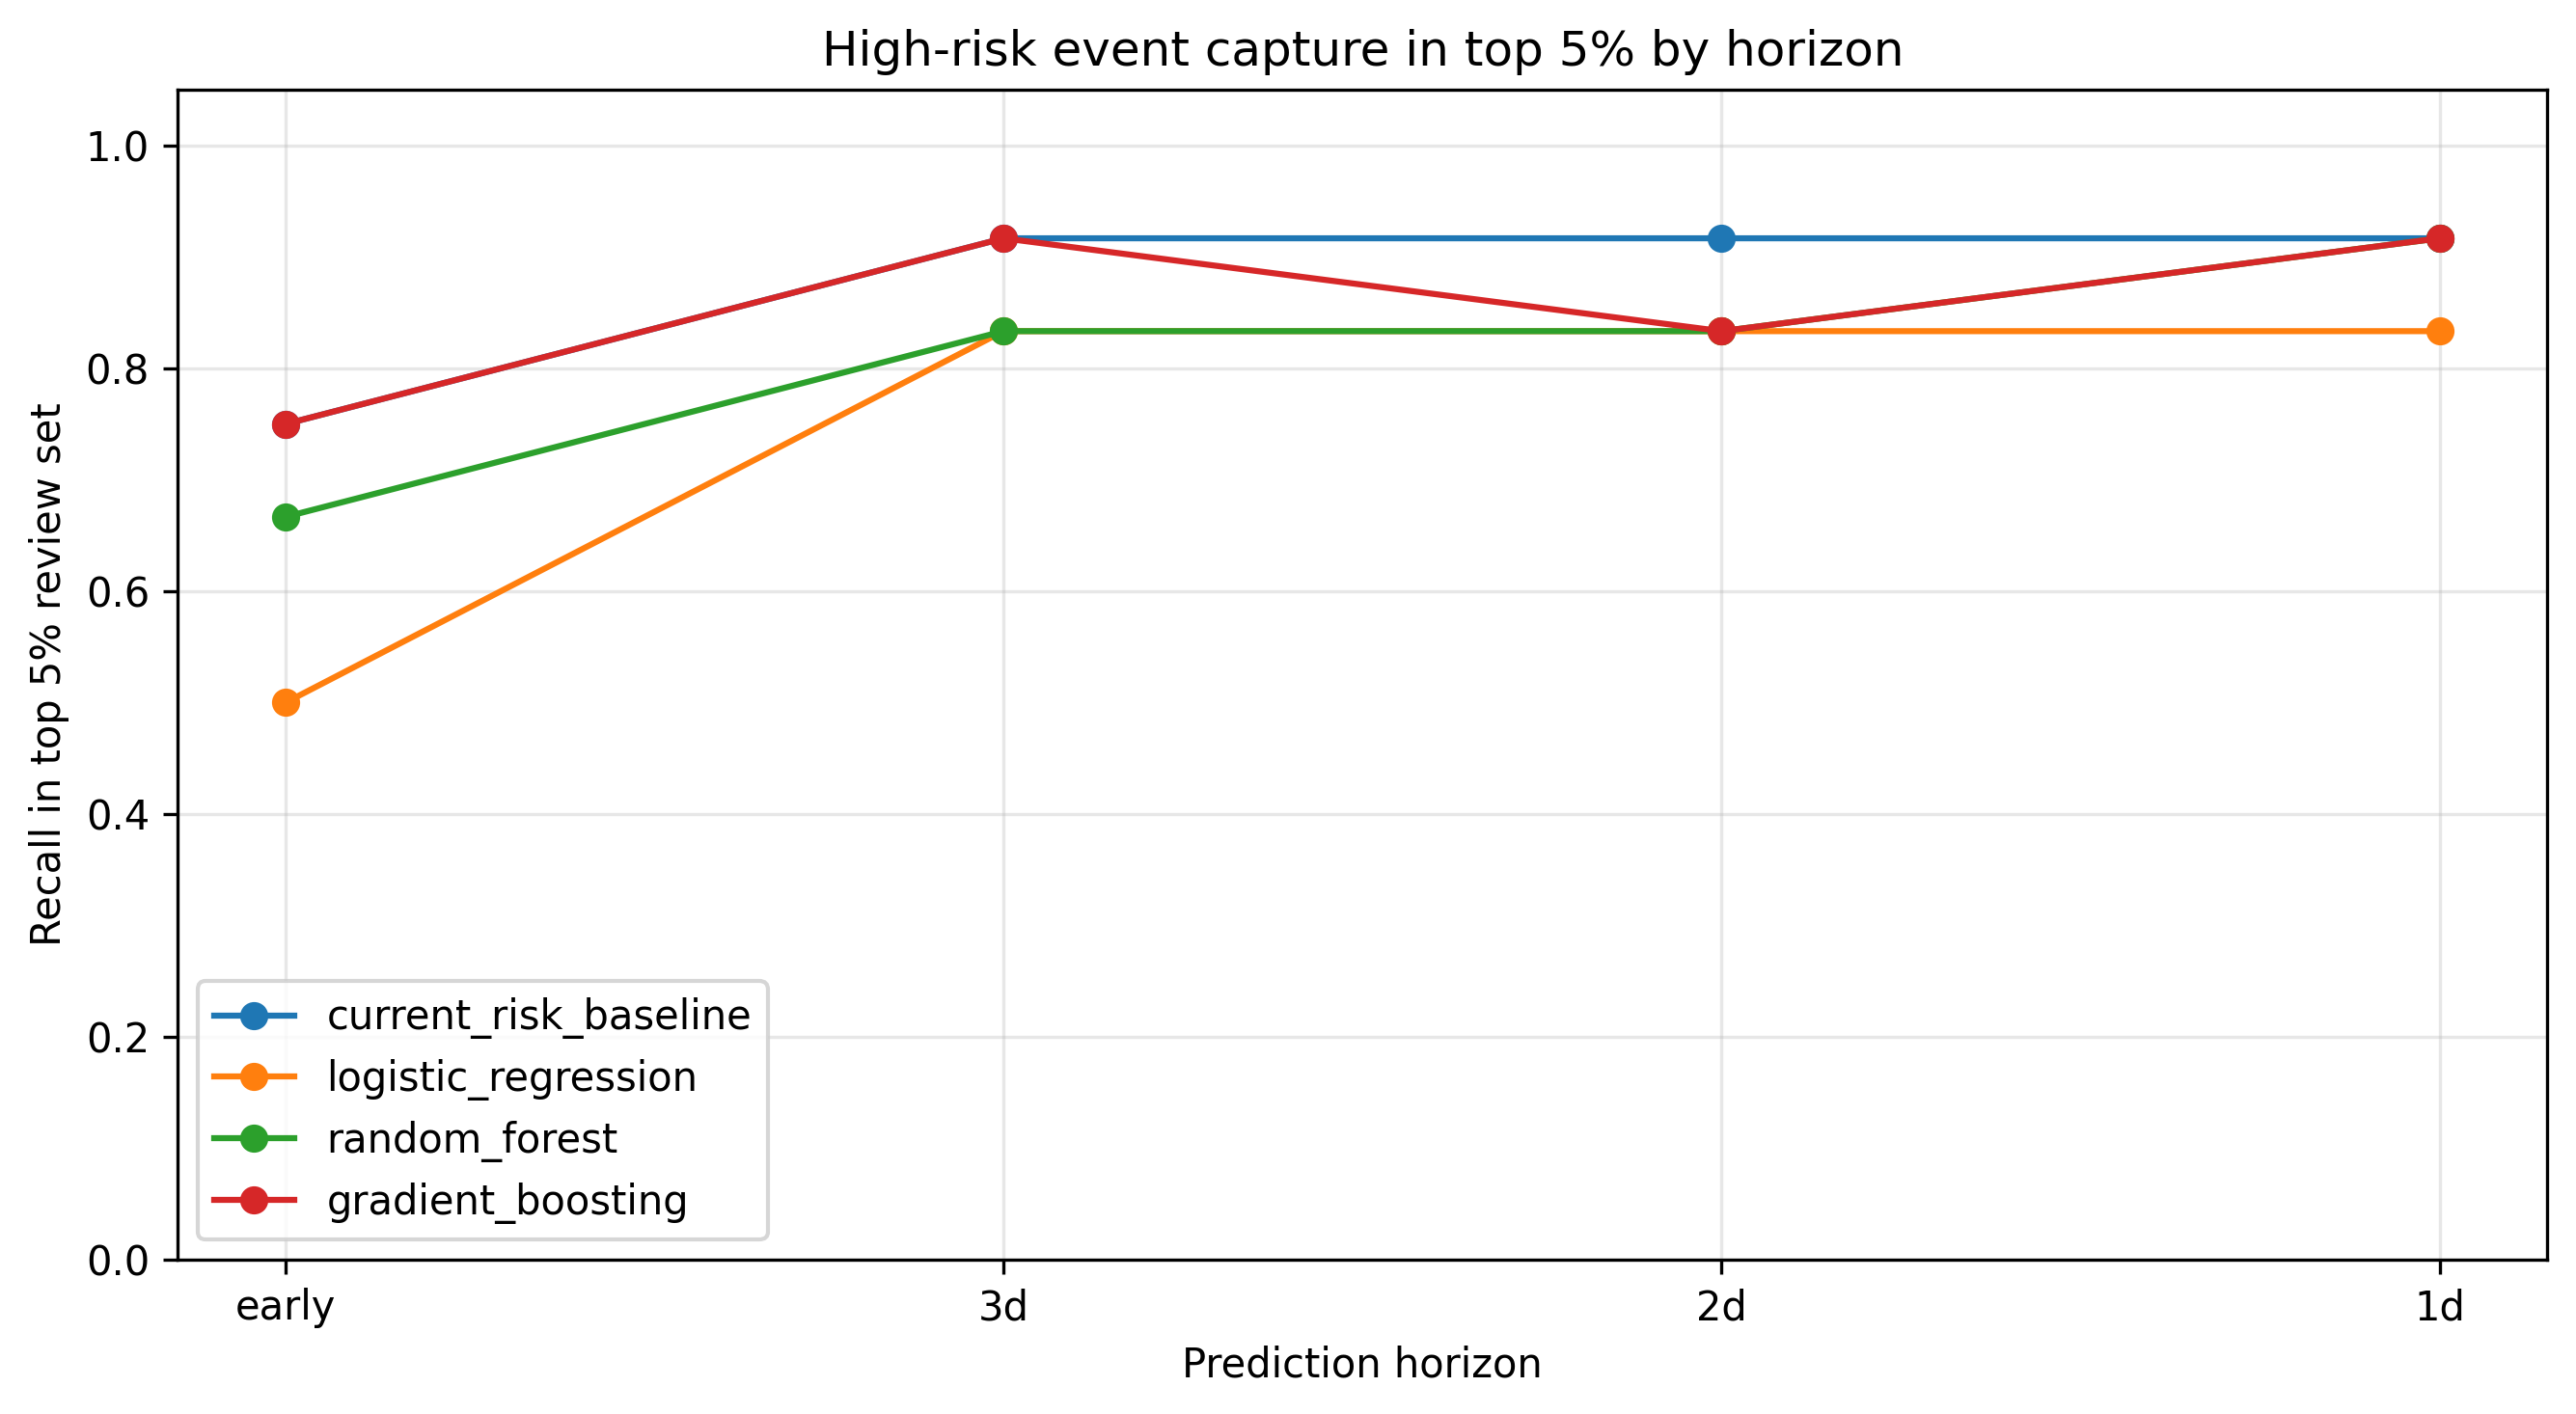
\includegraphics[width=\paperfigwidth]{top5_recall_by_horizon.png}
    \caption{Top-5\% recall by prediction horizon.}
    \label{fig:top5-horizon}
\end{figure}

Repeated split top-K results are strong. At the top 5\% review level, the bootstrap ensemble captures approximately 97.1\% of high-risk events at 1 day, 94.6\% at 2 days, 95.0\% at 3 days, and 71.3\% at the early horizon. This supports the framing of conjunction assessment as a ranking and prioritization problem rather than a standard classification problem.

\FloatBarrier

\subsection{Probability calibration}

Sigmoid calibration preserves ranking performance while improving probability quality. This is expected because calibration mostly adjusts the probability scale rather than changing the ordering of predictions.

\begin{figure}[!htbp]
    \centering
    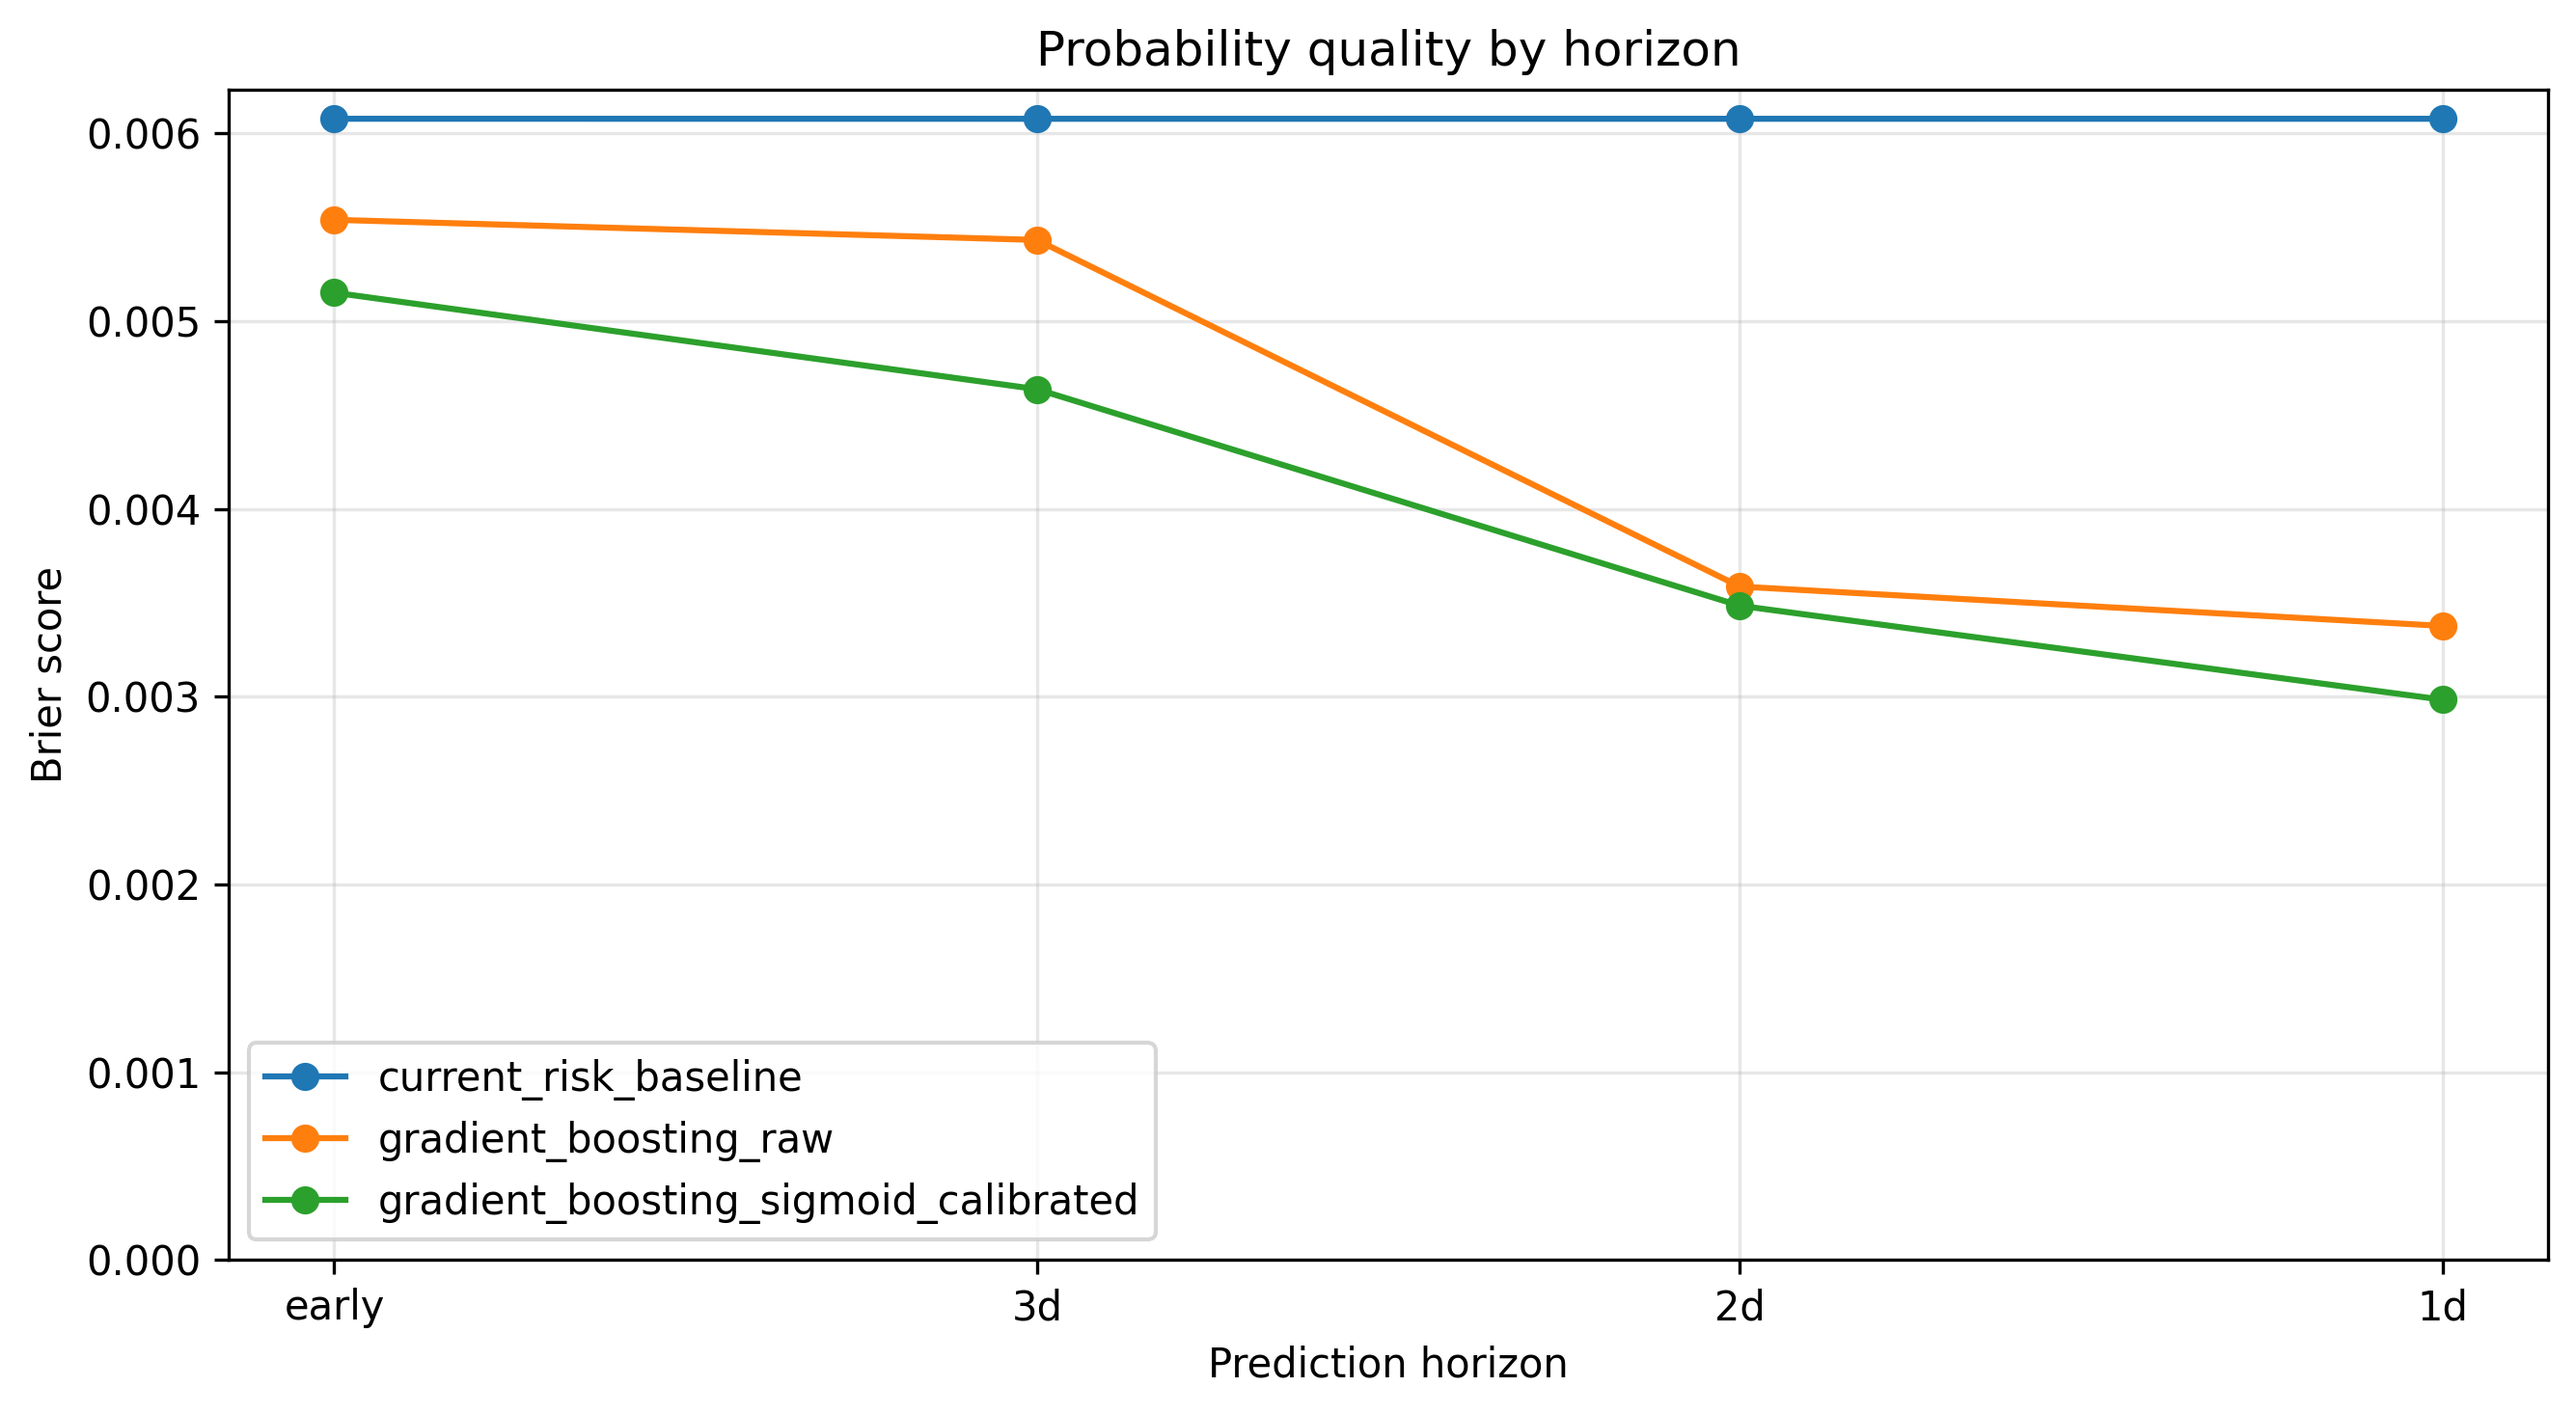
\includegraphics[width=\paperfigwidth]{brier_score_by_horizon.png}
    \caption{Brier score by prediction horizon.}
    \label{fig:brier}
\end{figure}

\begin{figure}[!htbp]
    \centering
    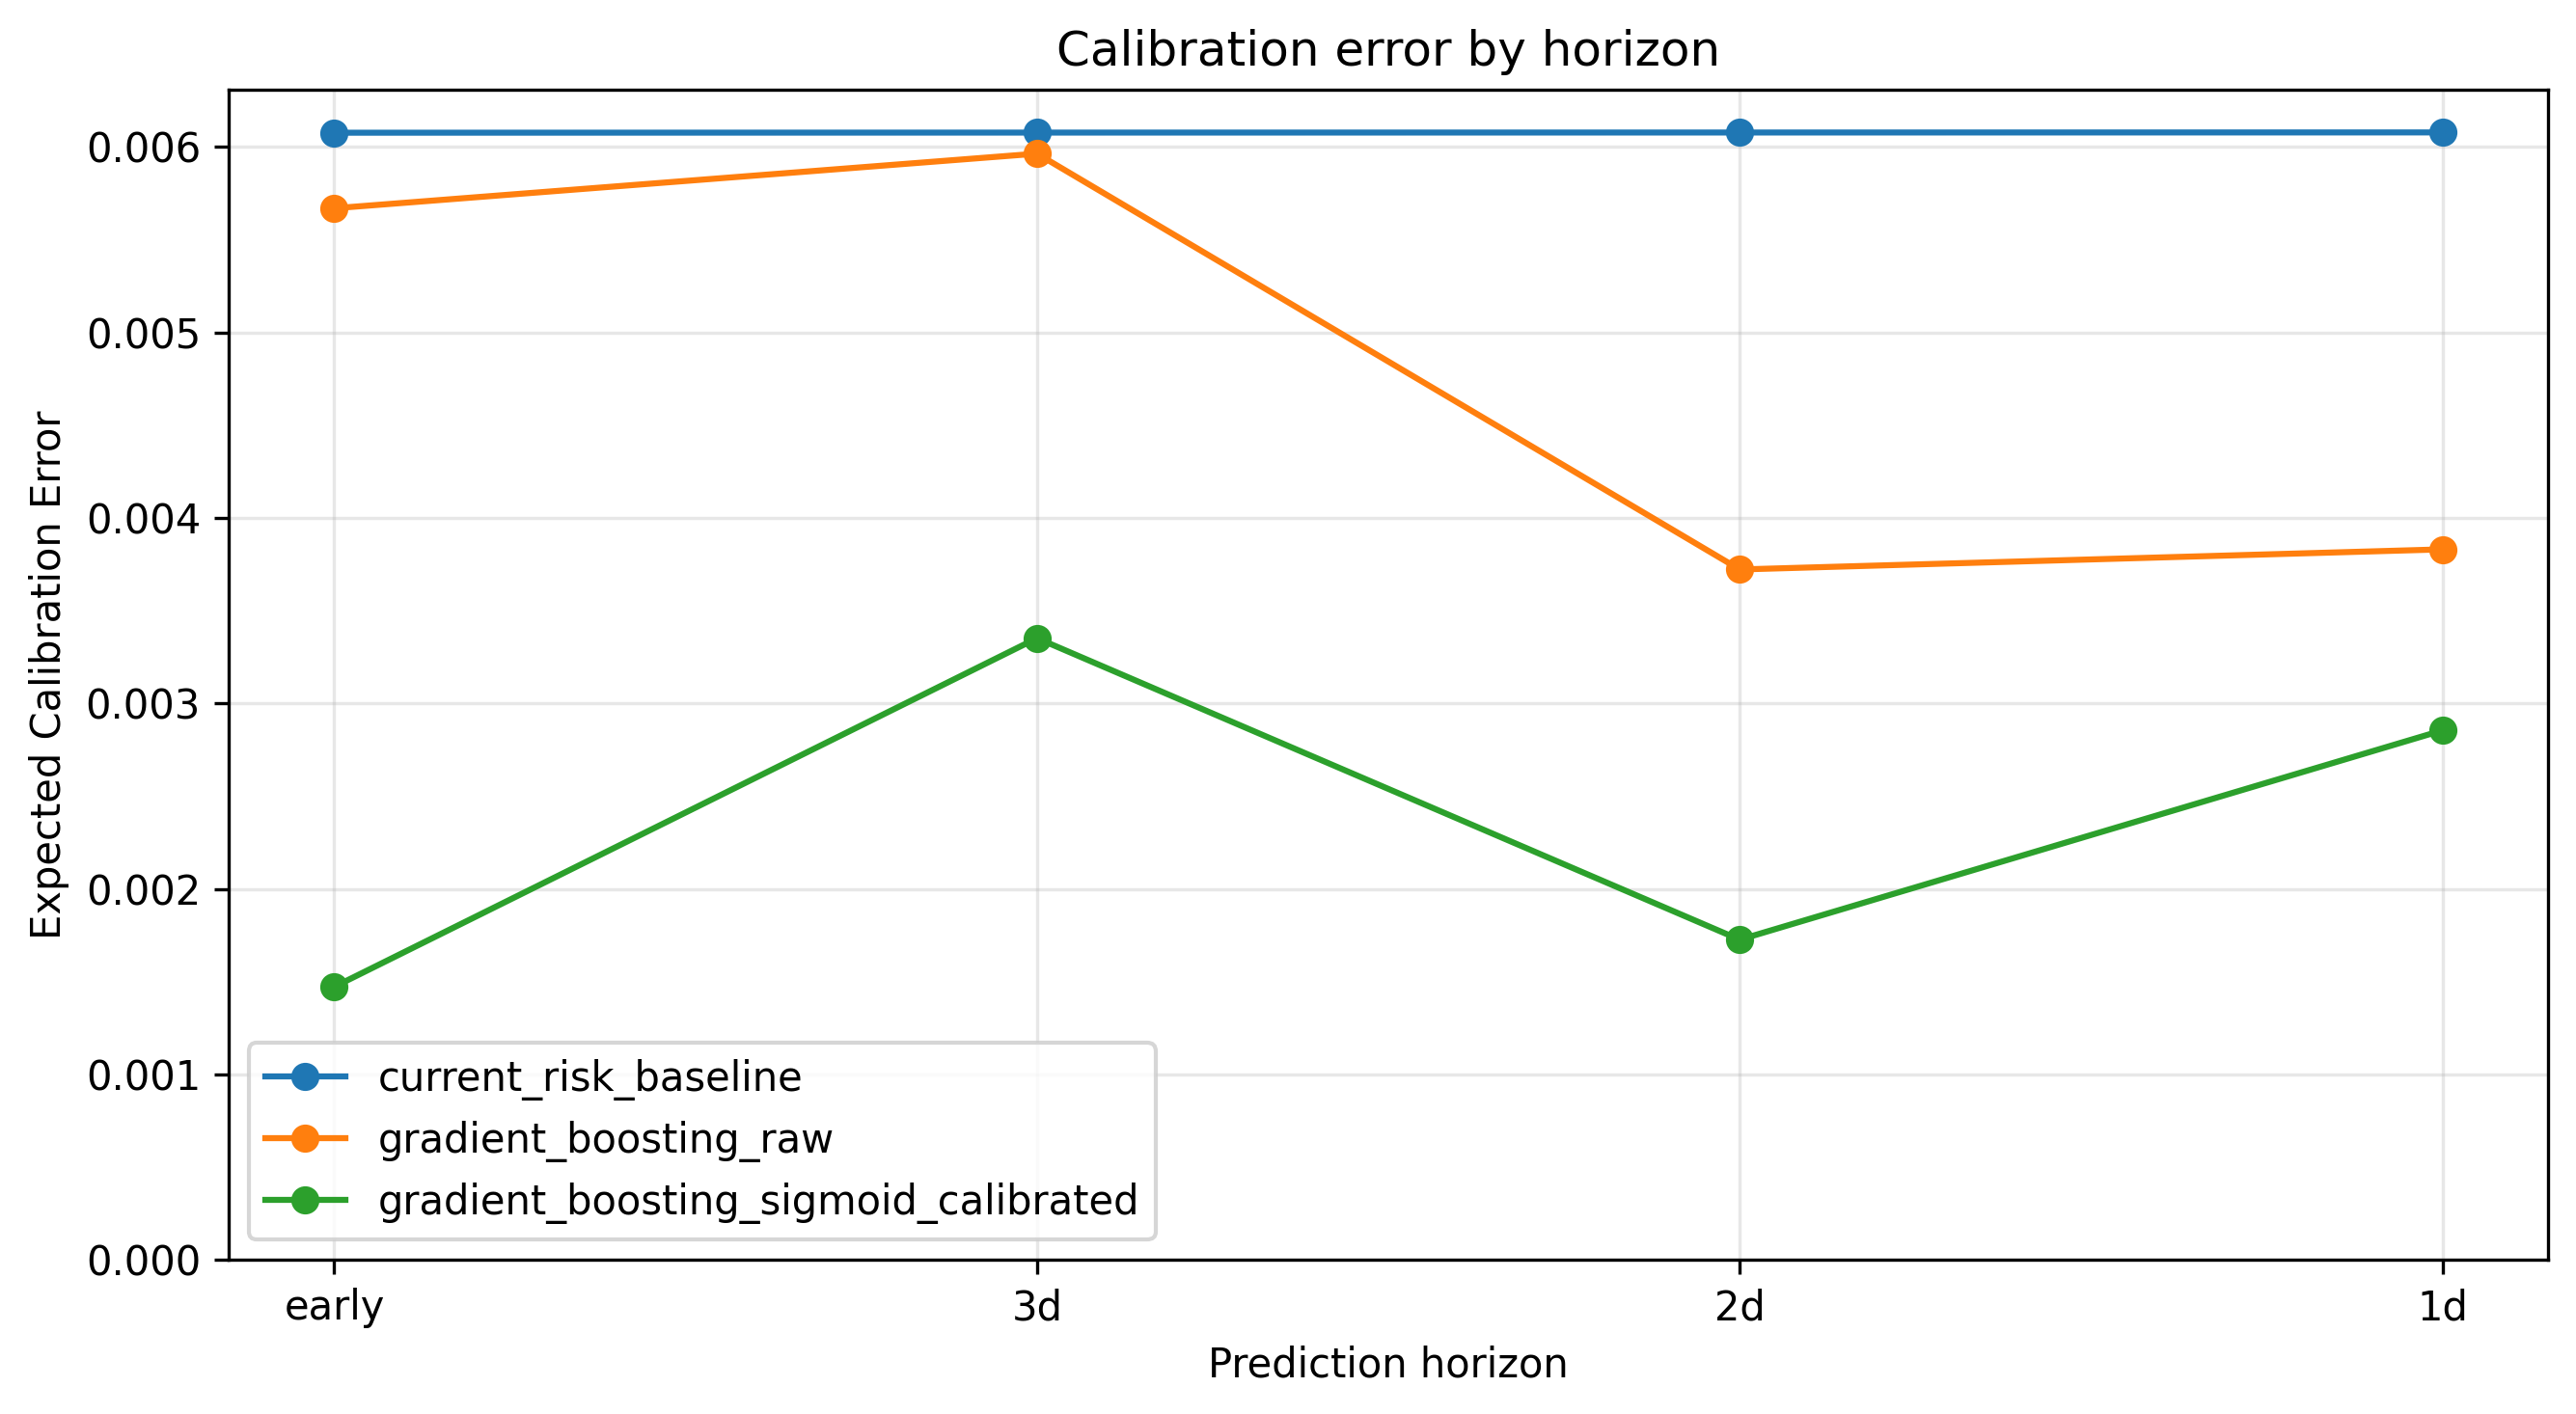
\includegraphics[width=\paperfigwidth]{ece_by_horizon.png}
    \caption{Expected Calibration Error by prediction horizon.}
    \label{fig:ece}
\end{figure}

Brier score and Expected Calibration Error improve after calibration across the evaluated horizons. This suggests that calibrated gradient boosting produces probabilities that are more useful for decision support than raw model outputs.

The quantile-binned reliability curves provide a clearer view of calibration in the rare-event setting.

\begin{figure}[!htbp]
    \centering
    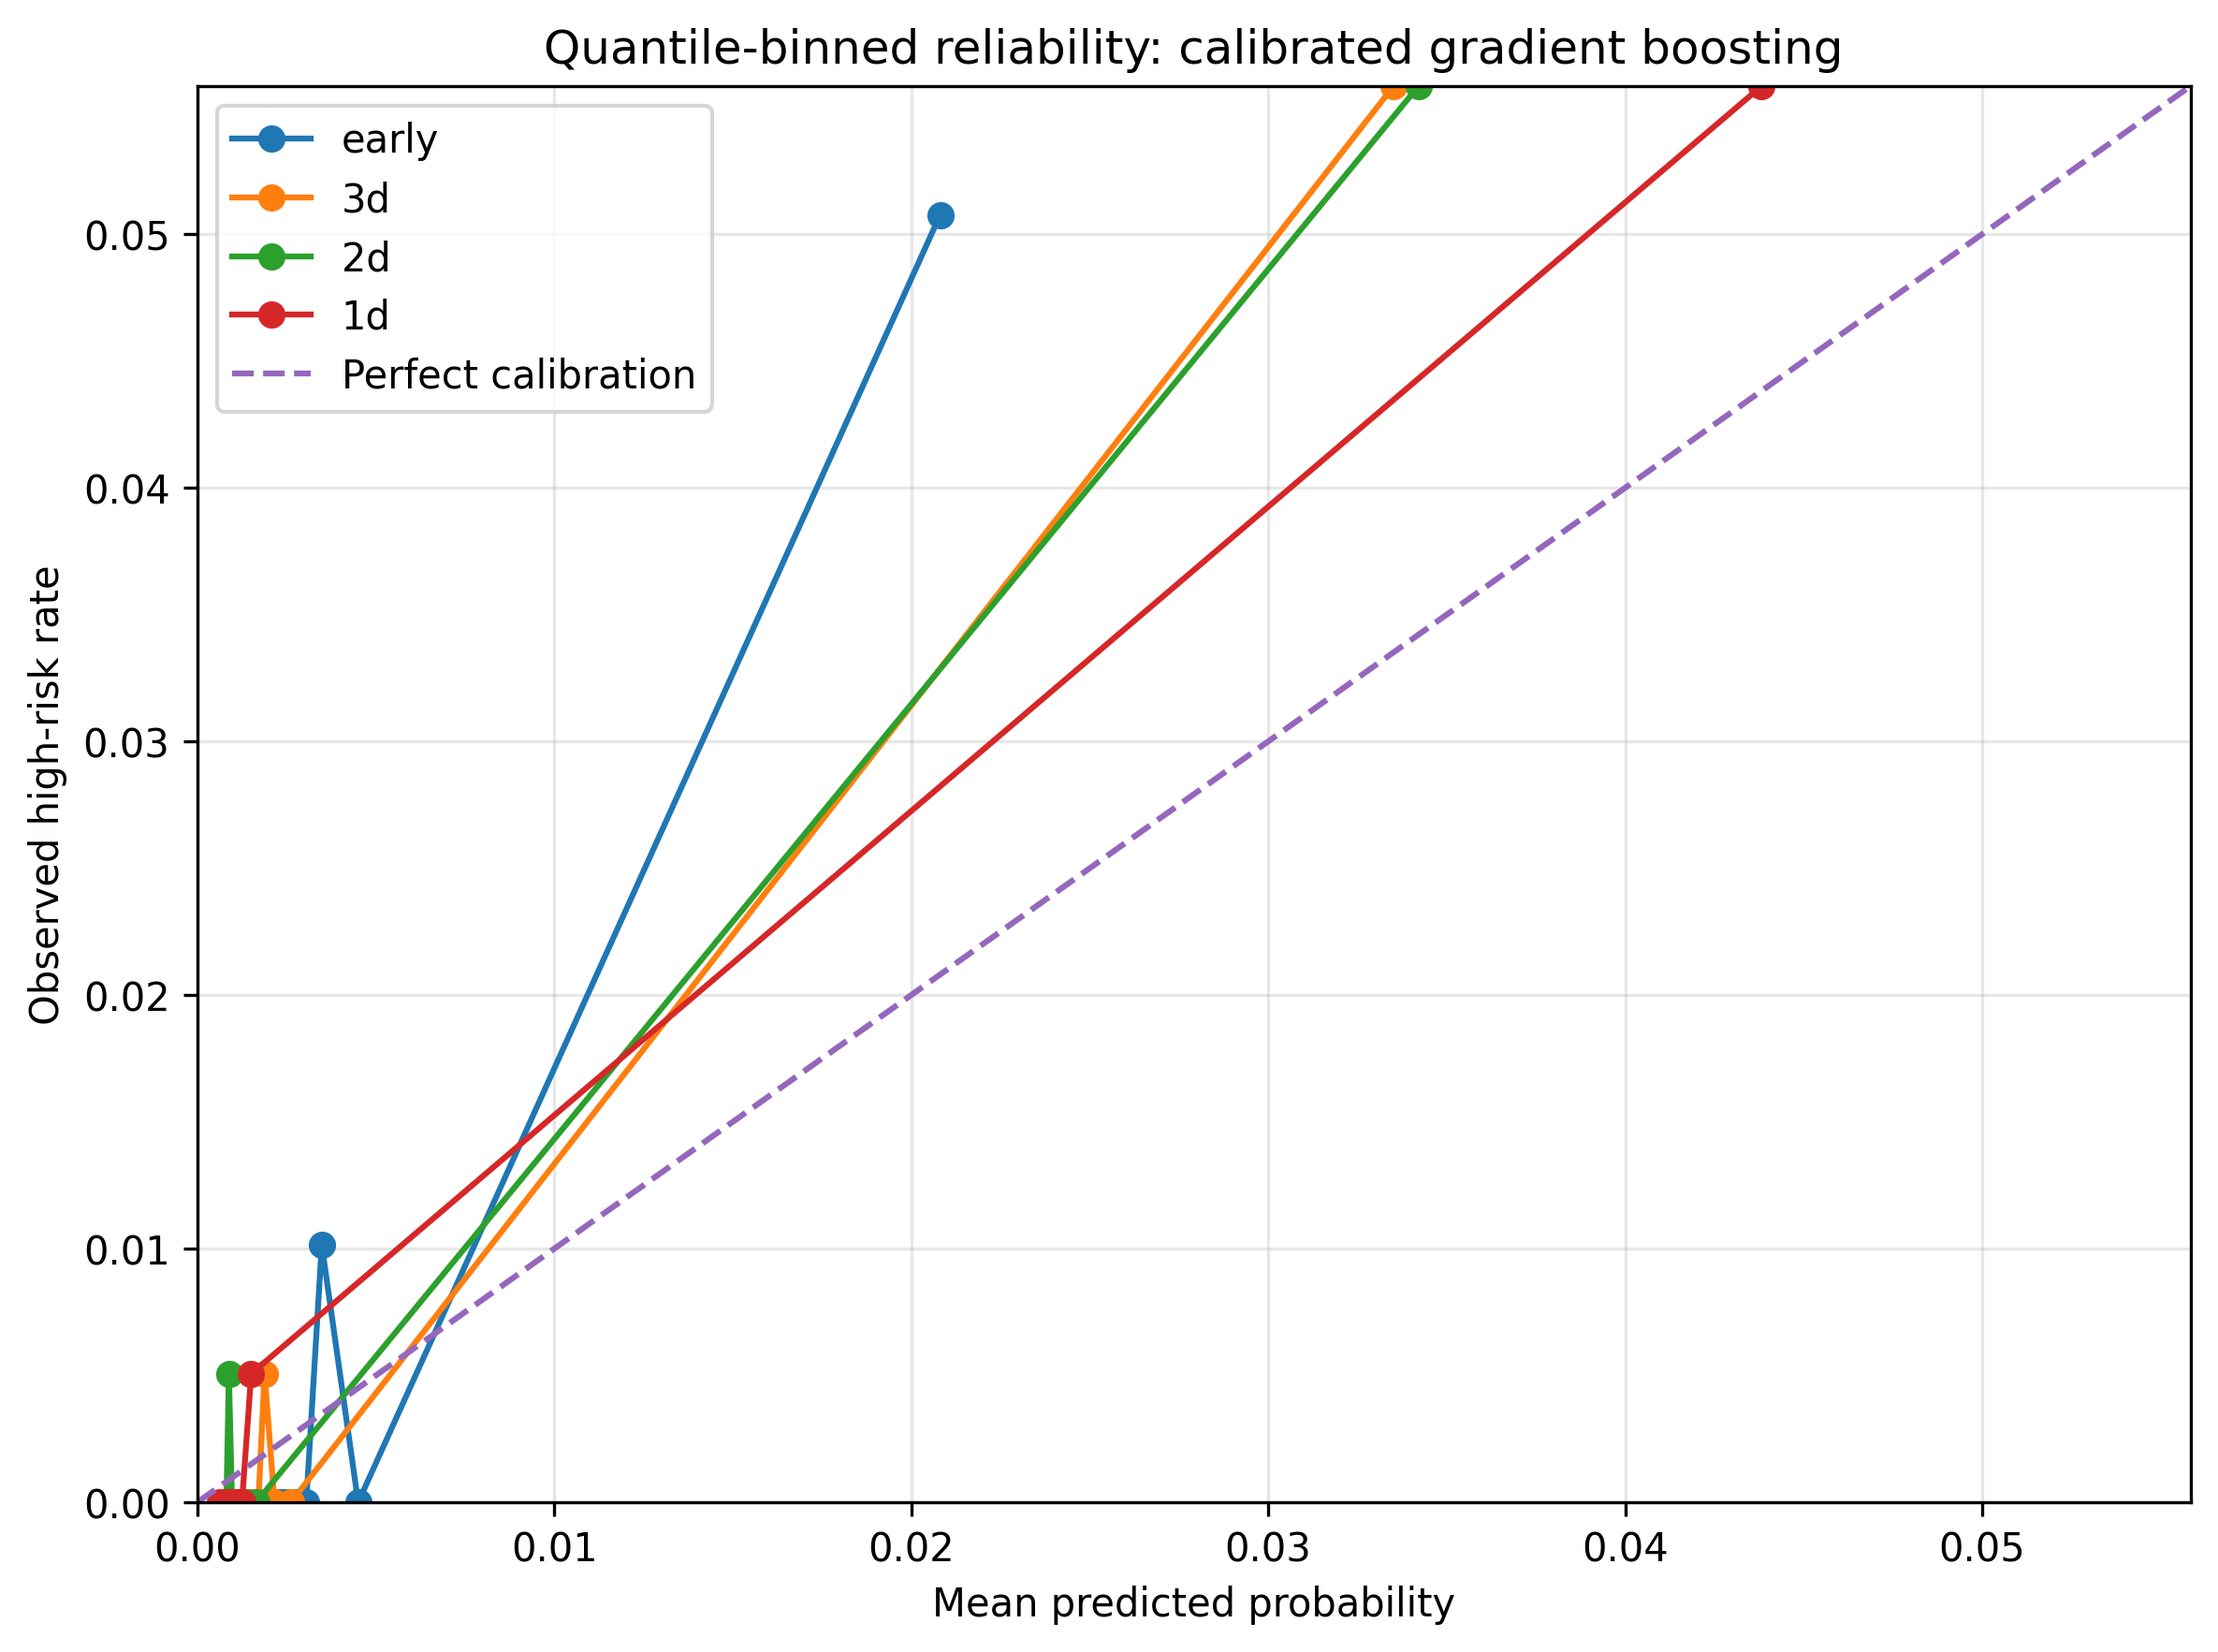
\includegraphics[width=\paperfigwidth]{quantile_reliability_by_horizon.png}
    \caption{Quantile-binned reliability by horizon.}
    \label{fig:reliability-horizon}
\end{figure}

The 1-day reliability comparison shows how the current-risk baseline, raw gradient boosting, and calibrated gradient boosting differ in probability behavior.

\begin{figure}[!htbp]
    \centering
    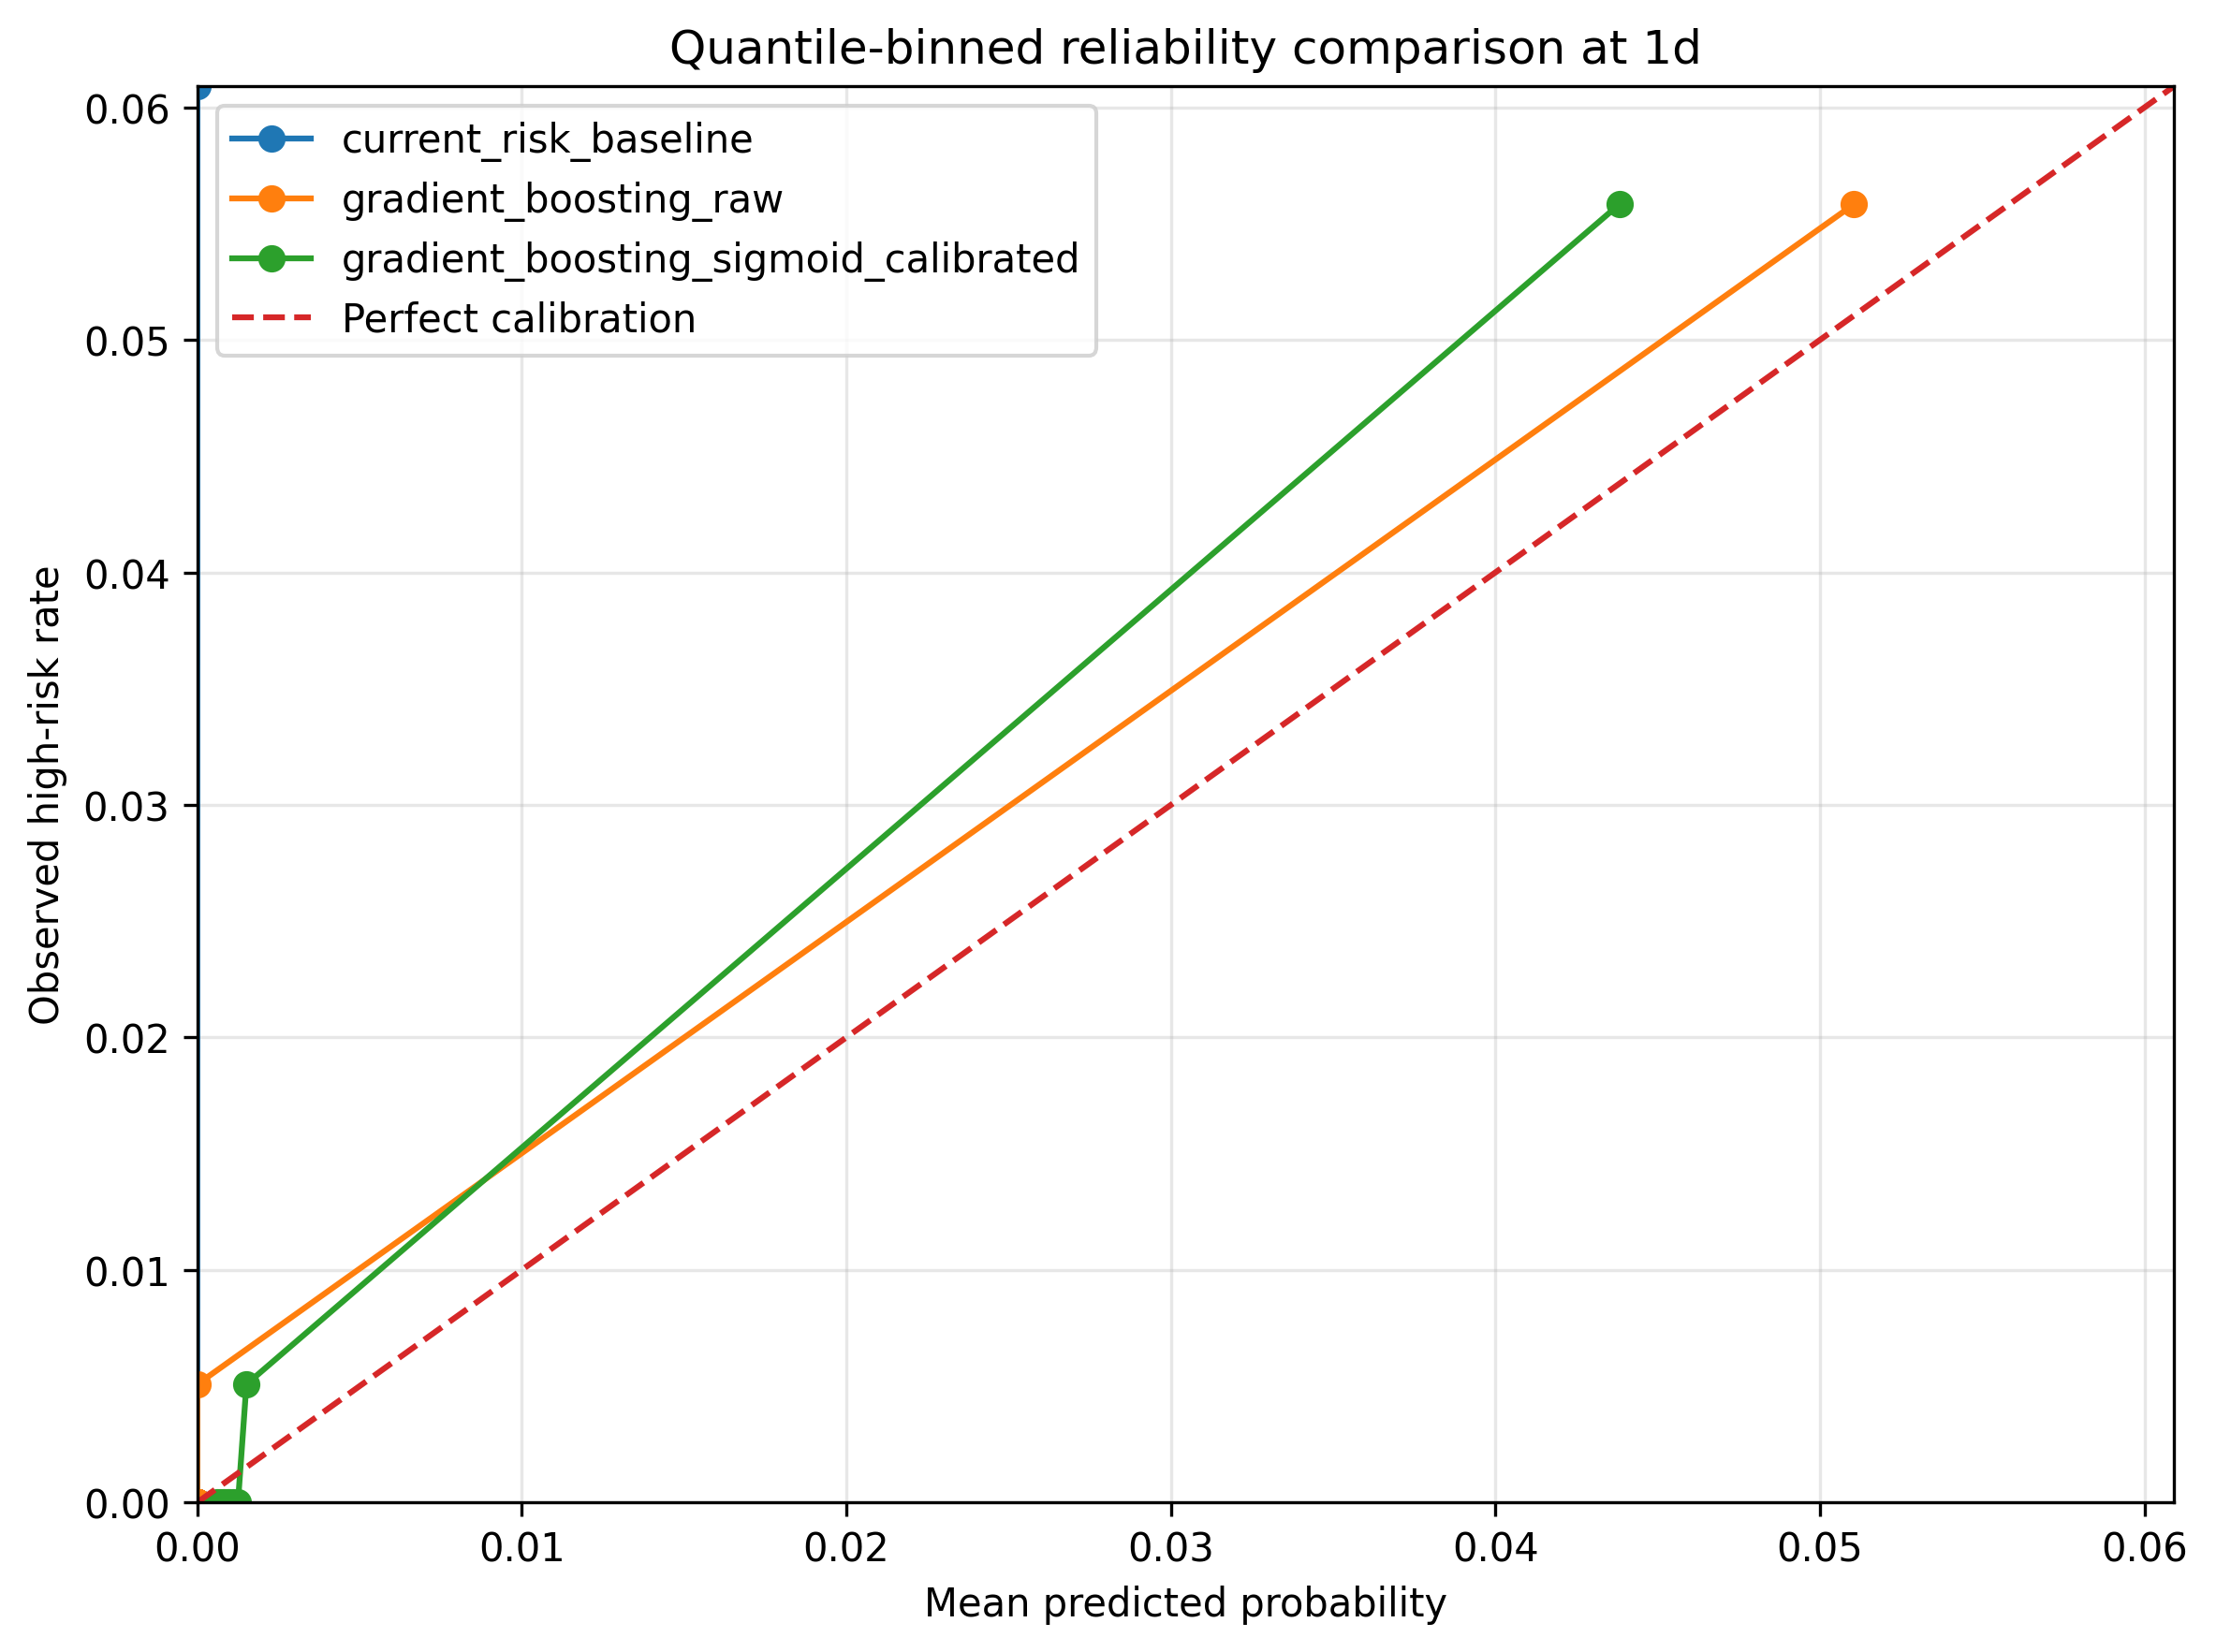
\includegraphics[width=\paperfigwidth]{quantile_reliability_comparison_1d.png}
    \caption{Quantile-binned reliability comparison at 1 day.}
    \label{fig:reliability-1d}
\end{figure}

\FloatBarrier

\subsection{Uncertainty-aware escalation}

Bootstrap ensemble uncertainty is strongly concentrated on high-risk events. High-risk events have much larger predictive standard deviation than non-high-risk events.

\begin{figure}[!htbp]
    \centering
    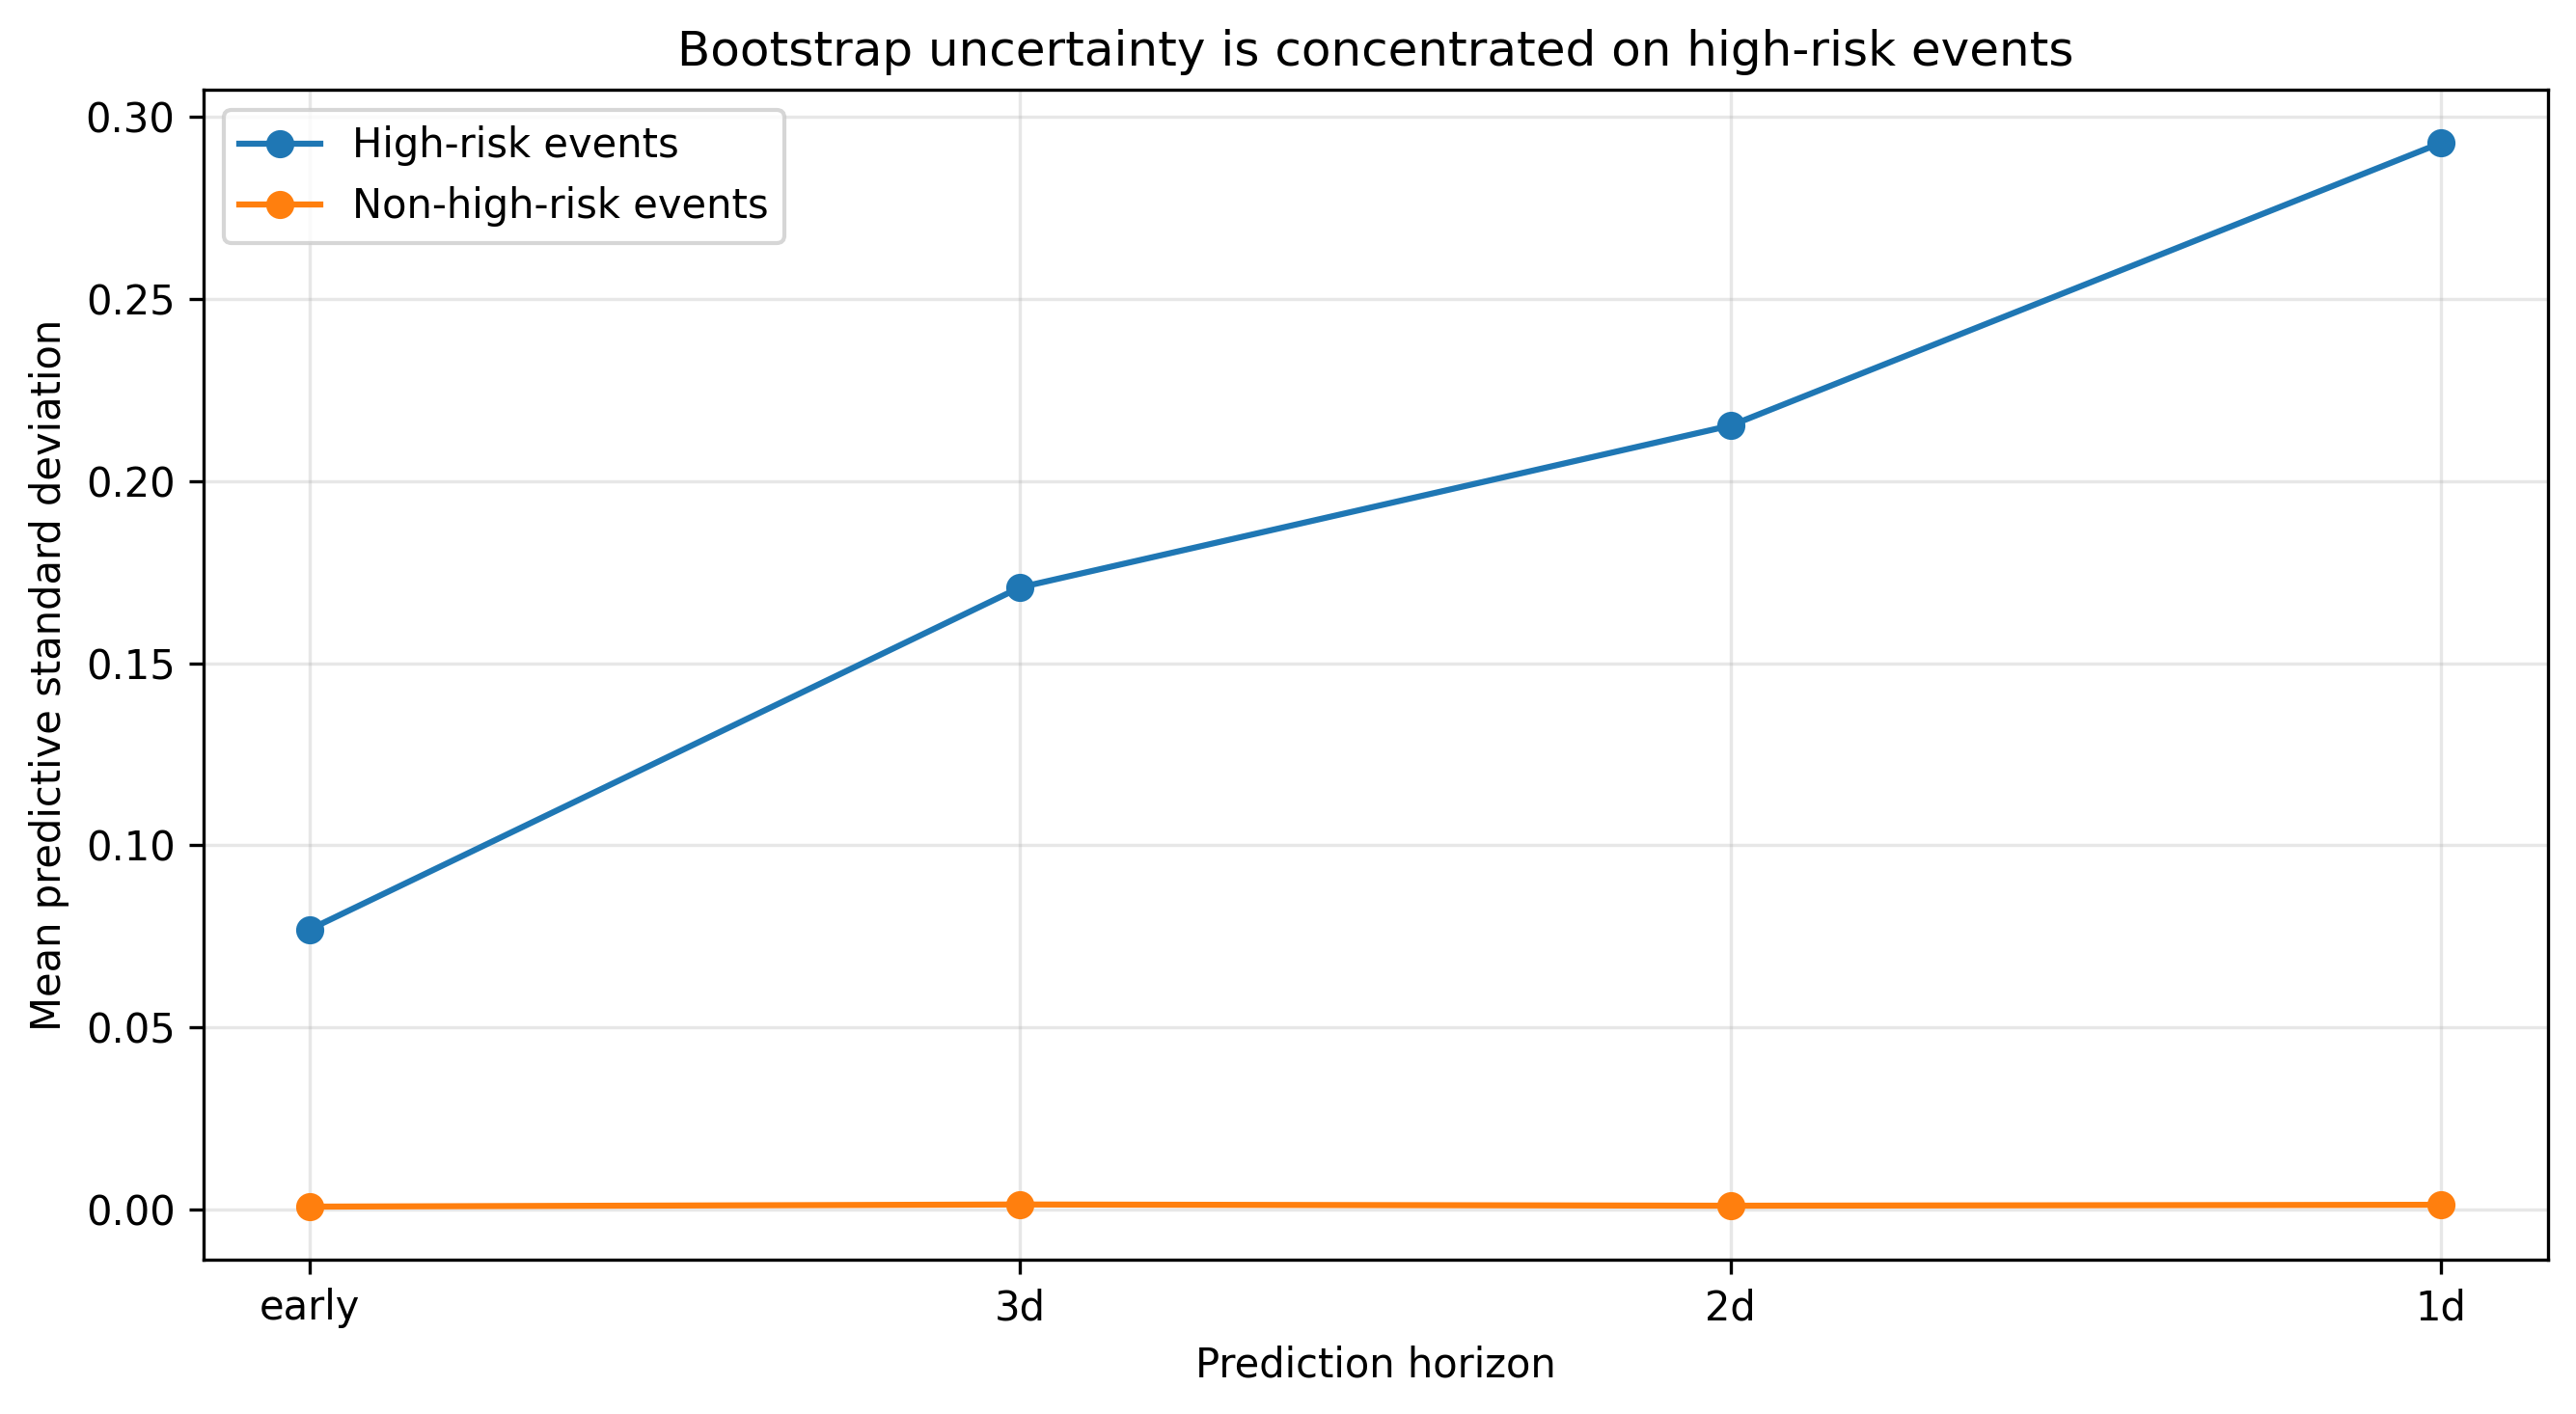
\includegraphics[width=\paperfigwidth]{uncertainty_positive_vs_negative.png}
    \caption{Predictive uncertainty for high-risk versus non-high-risk events.}
    \label{fig:uncertainty-pos-neg}
\end{figure}

This result suggests that uncertainty itself is a useful triage signal. The model is not merely assigning higher risk to some events; it is also expressing greater uncertainty on events that are more likely to matter.

\begin{figure}[!htbp]
    \centering
    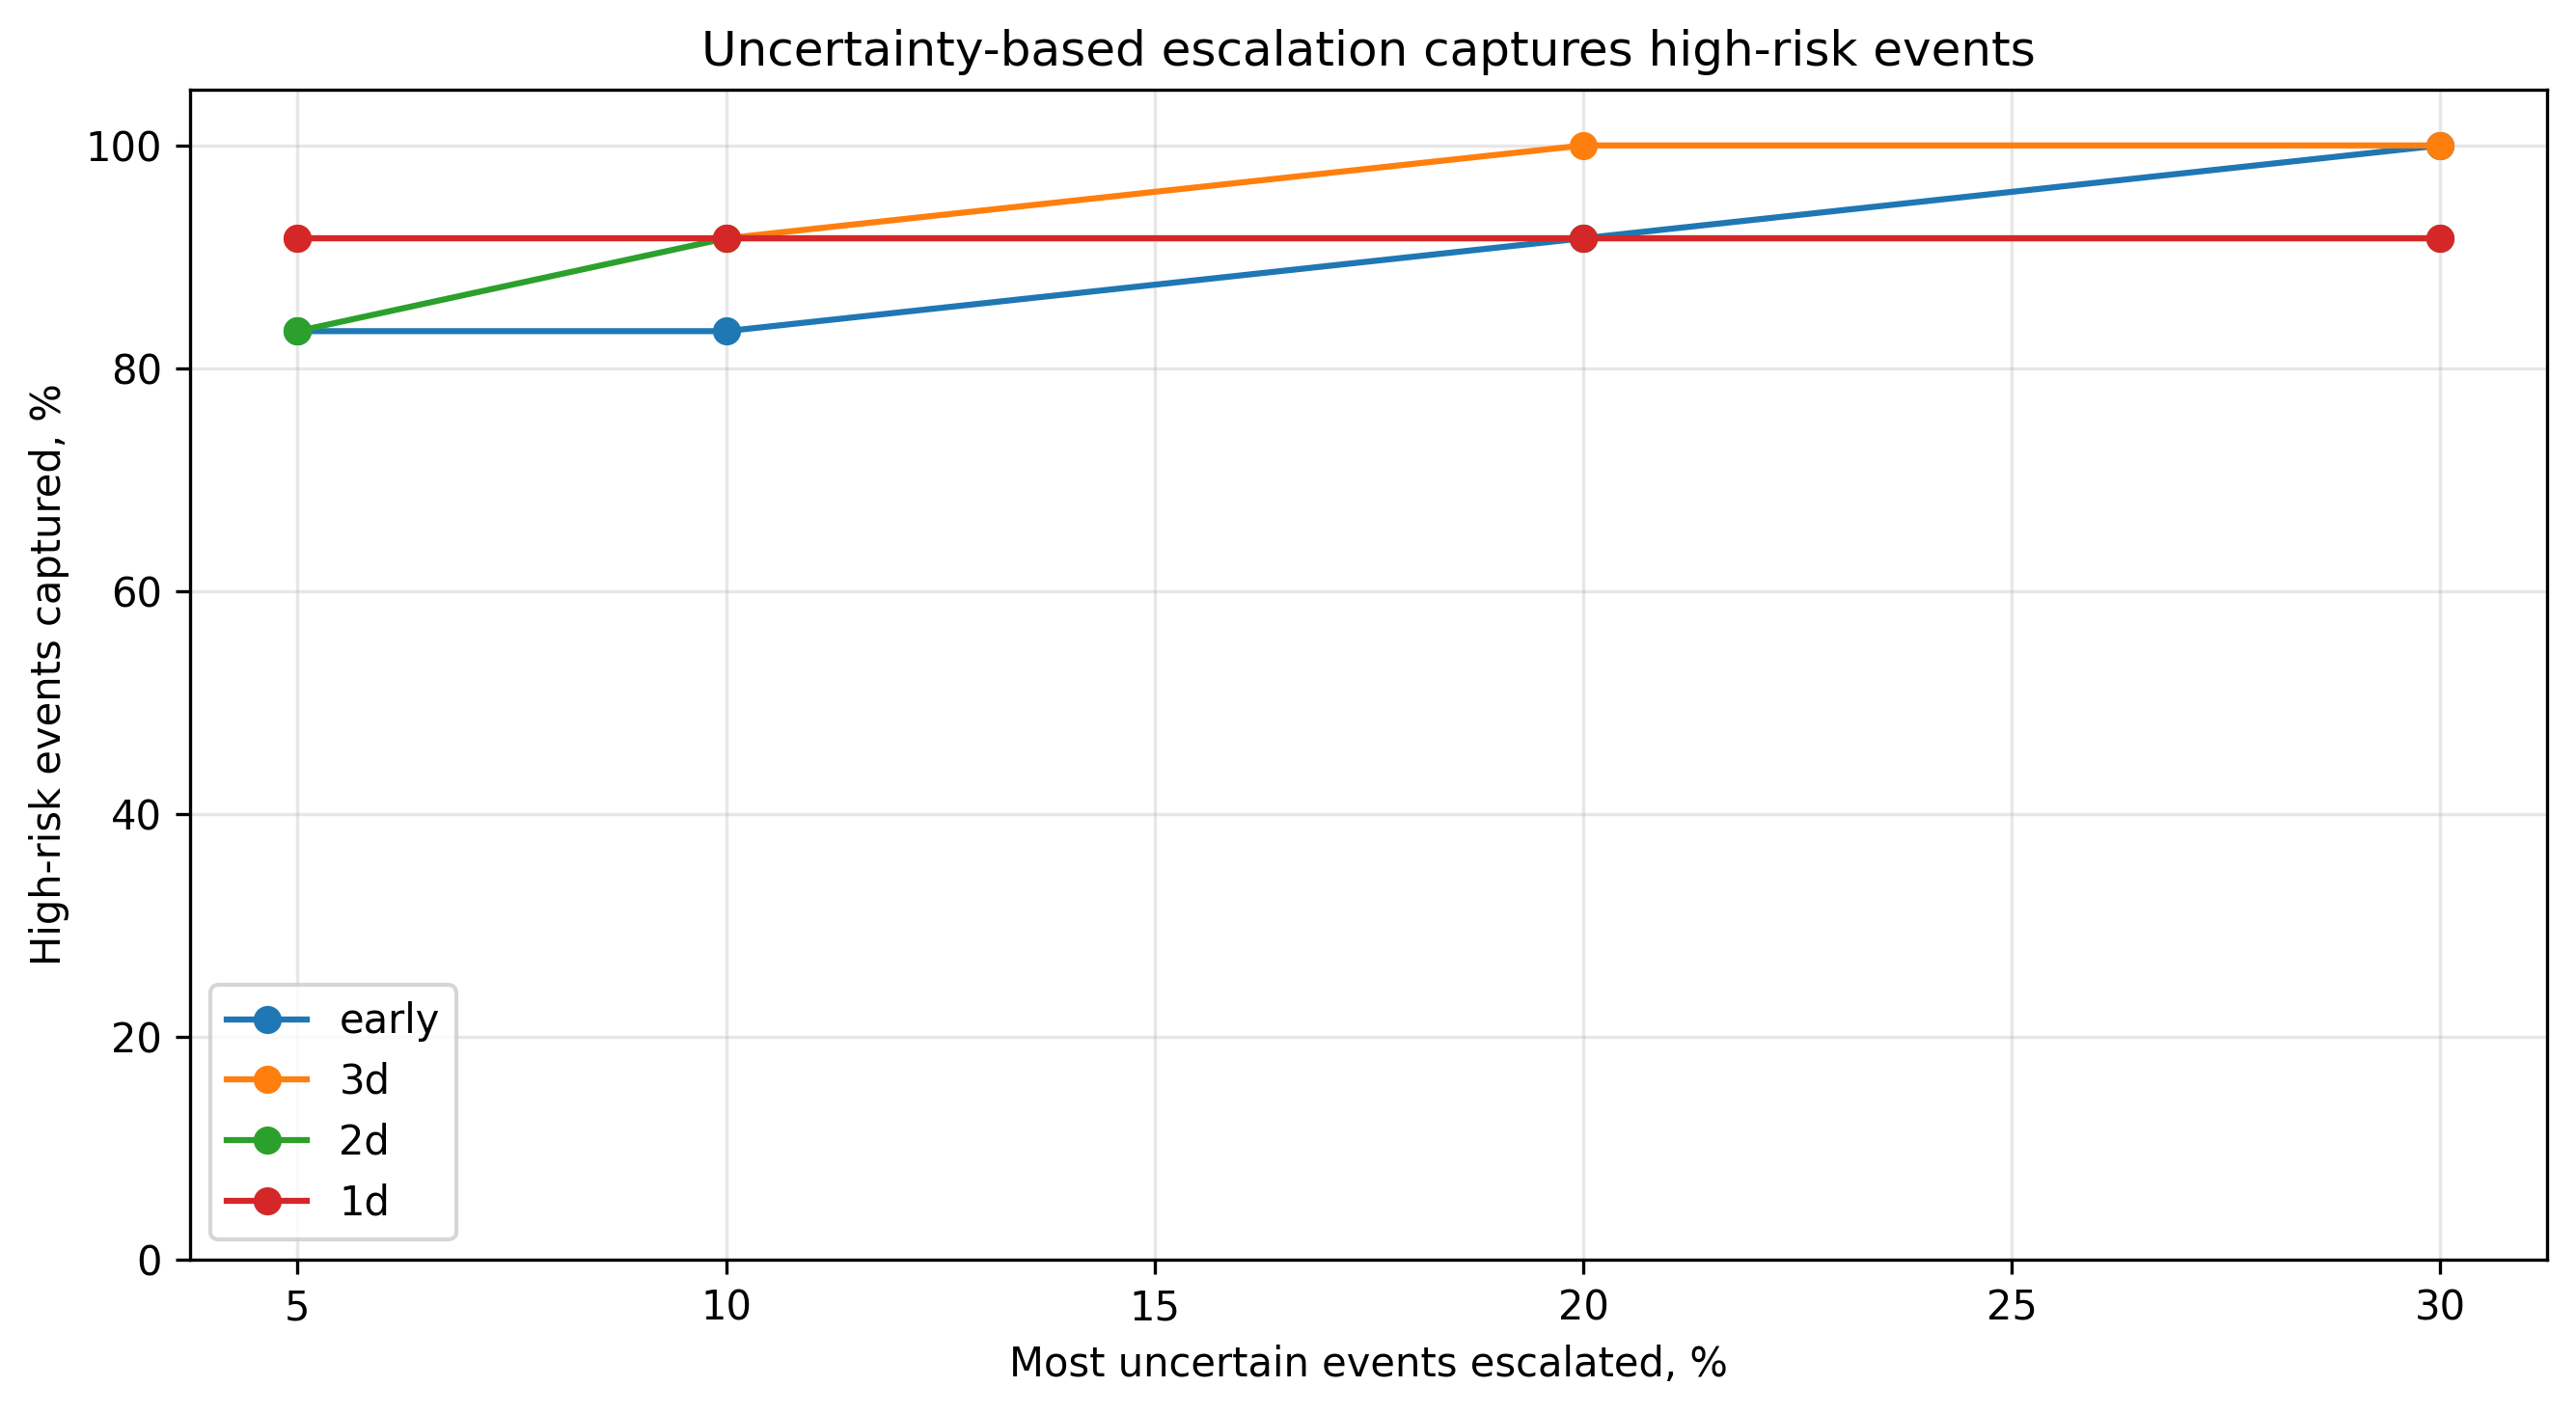
\includegraphics[width=\paperfigwidth]{positive_escalation_rate.png}
    \caption{Positive escalation rate from uncertainty-based review.}
    \label{fig:positive-escalation}
\end{figure}

Across 20 repeated event-level splits, uncertainty-based escalation substantially outperforms random escalation. At the 10\% escalation level, uncertainty captures the rates shown in Table~\ref{tab:escalation}.

\begin{table}[!htbp]
\centering
\caption{High-risk events captured at 10\% escalation. Values are mean $\pm$ standard deviation across 20 event-level splits.}
\label{tab:escalation}
\begin{tabular}{lccc}
\toprule
Horizon & Uncertainty escalation & Current-risk escalation & Random escalation \\
\midrule
1d & $97.5\% \pm 3.9\%$ & $99.6\% \pm 1.9\%$ & $8.3\% \pm 7.2\%$ \\
2d & $96.3\% \pm 4.3\%$ & $97.9\% \pm 3.7\%$ & $9.6\% \pm 7.8\%$ \\
3d & $97.5\% \pm 3.9\%$ & $97.9\% \pm 3.7\%$ & $11.3\% \pm 10.2\%$ \\
Early & $80.8\% \pm 9.8\%$ & $84.6\% \pm 7.8\%$ & $8.3\% \pm 6.6\%$ \\
\bottomrule
\end{tabular}
\end{table}

\begin{figure}[!htbp]
    \centering
    \includegraphics[width=\paperfigwidth]{repeated_split_escalation_10pct.png}
    \caption{Repeated split 10\% escalation robustness.}
    \label{fig:escalation-10pct}
\end{figure}

The coverage tradeoff shows how many high-risk events are escalated as the automated coverage rate decreases.

\begin{figure}[!htbp]
    \centering
    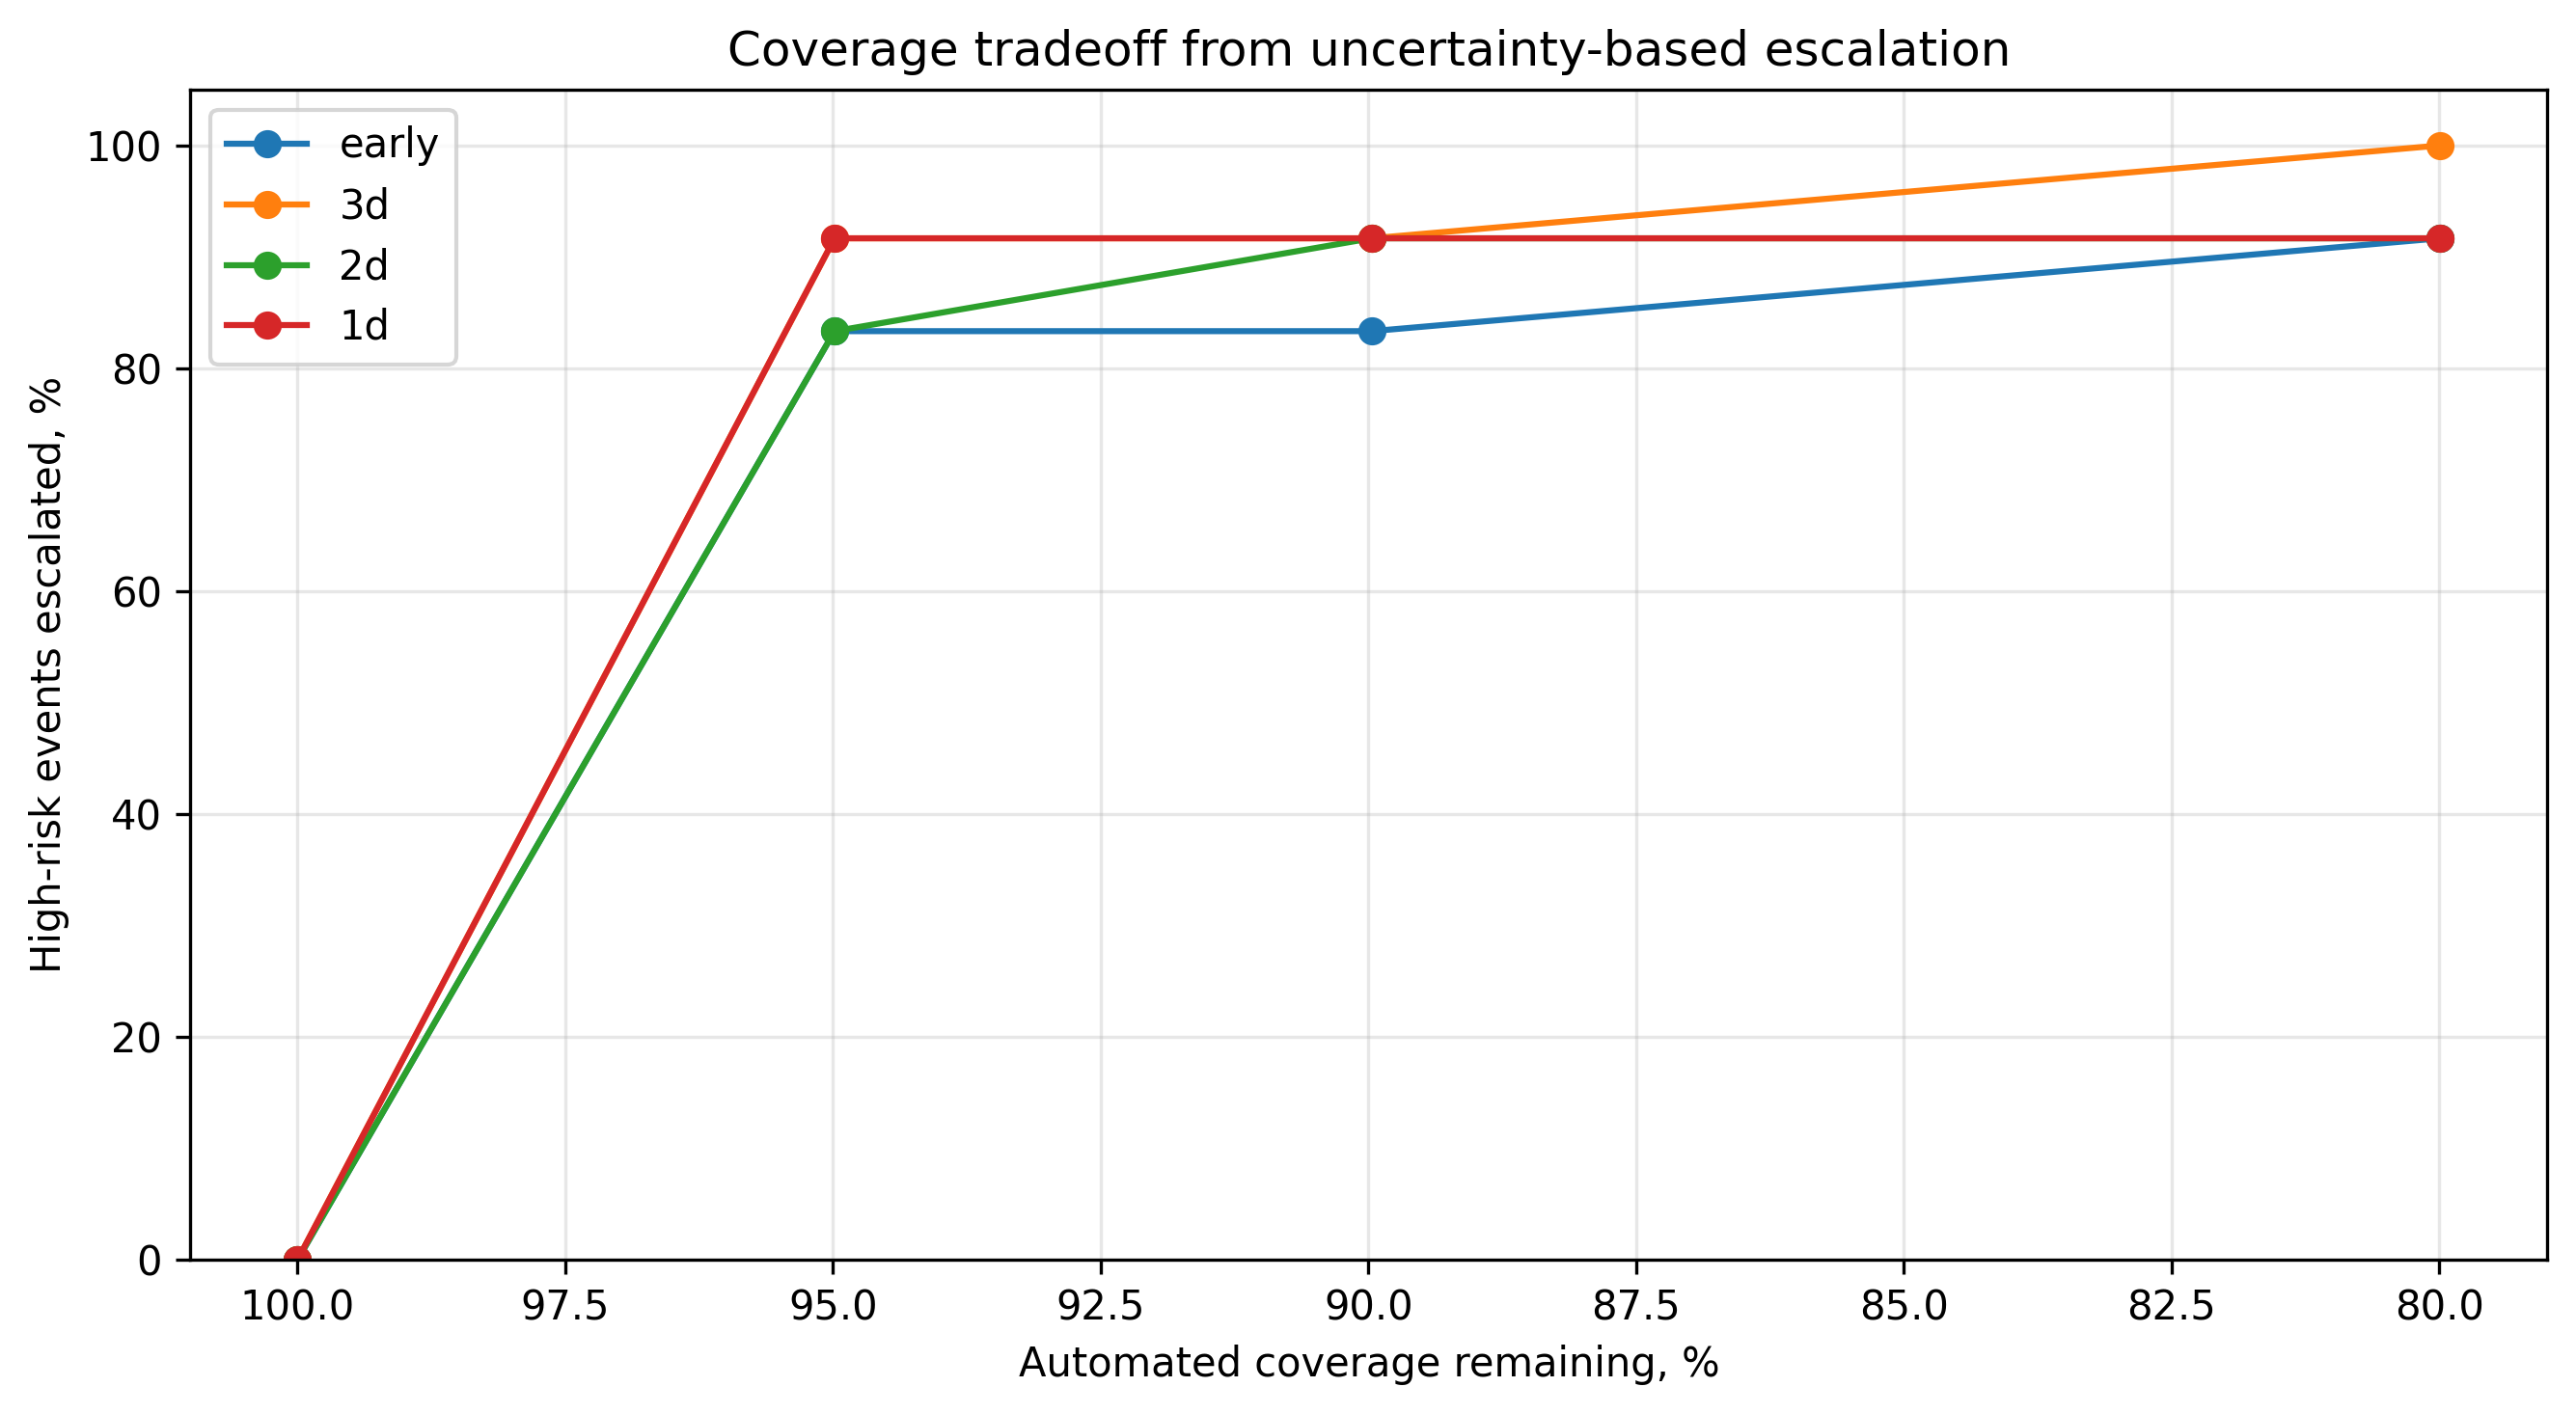
\includegraphics[width=\paperfigwidth]{uncertainty_abstention_coverage.png}
    \caption{Uncertainty abstention coverage tradeoff.}
    \label{fig:coverage-tradeoff}
\end{figure}

These results should not be interpreted as showing that uncertainty replaces current risk. Current-risk escalation remains an extremely strong baseline, especially near TCA. Instead, the repeated split results support a more careful claim: uncertainty is a complementary human-review signal that performs far above random escalation and remains competitive with current-risk escalation.

\FloatBarrier

\subsection{Current-risk feature ablation}

The current-risk feature ablation clarifies the source of the learned model's ranking gains. Gradient boosting with the current risk feature outperforms direct current-risk ranking in PR-AUC at every horizon. Removing the current risk feature reduces gradient-boosting PR-AUC at every horizon, but the no-risk model still exceeds direct current-risk PR-AUC.

\begin{table}[!htbp]
\centering
\caption{Current-risk feature ablation. Values are mean $\pm$ standard deviation across 20 event-level splits.}
\label{tab:risk-ablation}
\resizebox{\textwidth}{!}{%
\begin{tabular}{lccccc}
\toprule
Horizon & Current risk & GB + risk & GB $-$ risk & GB + risk $-$ current & GB + risk $-$ no risk \\
\midrule
1d & $0.581 \pm 0.085$ & $0.739 \pm 0.096$ & $0.634 \pm 0.147$ & $+0.158 \pm 0.119$ & $+0.105 \pm 0.132$ \\
2d & $0.367 \pm 0.083$ & $0.610 \pm 0.129$ & $0.439 \pm 0.107$ & $+0.243 \pm 0.086$ & $+0.171 \pm 0.102$ \\
3d & $0.237 \pm 0.048$ & $0.493 \pm 0.090$ & $0.379 \pm 0.089$ & $+0.257 \pm 0.102$ & $+0.114 \pm 0.127$ \\
Early & $0.109 \pm 0.031$ & $0.233 \pm 0.082$ & $0.180 \pm 0.066$ & $+0.123 \pm 0.077$ & $+0.052 \pm 0.061$ \\
\bottomrule
\end{tabular}}
\end{table}

\begin{figure}[!htbp]
    \centering
    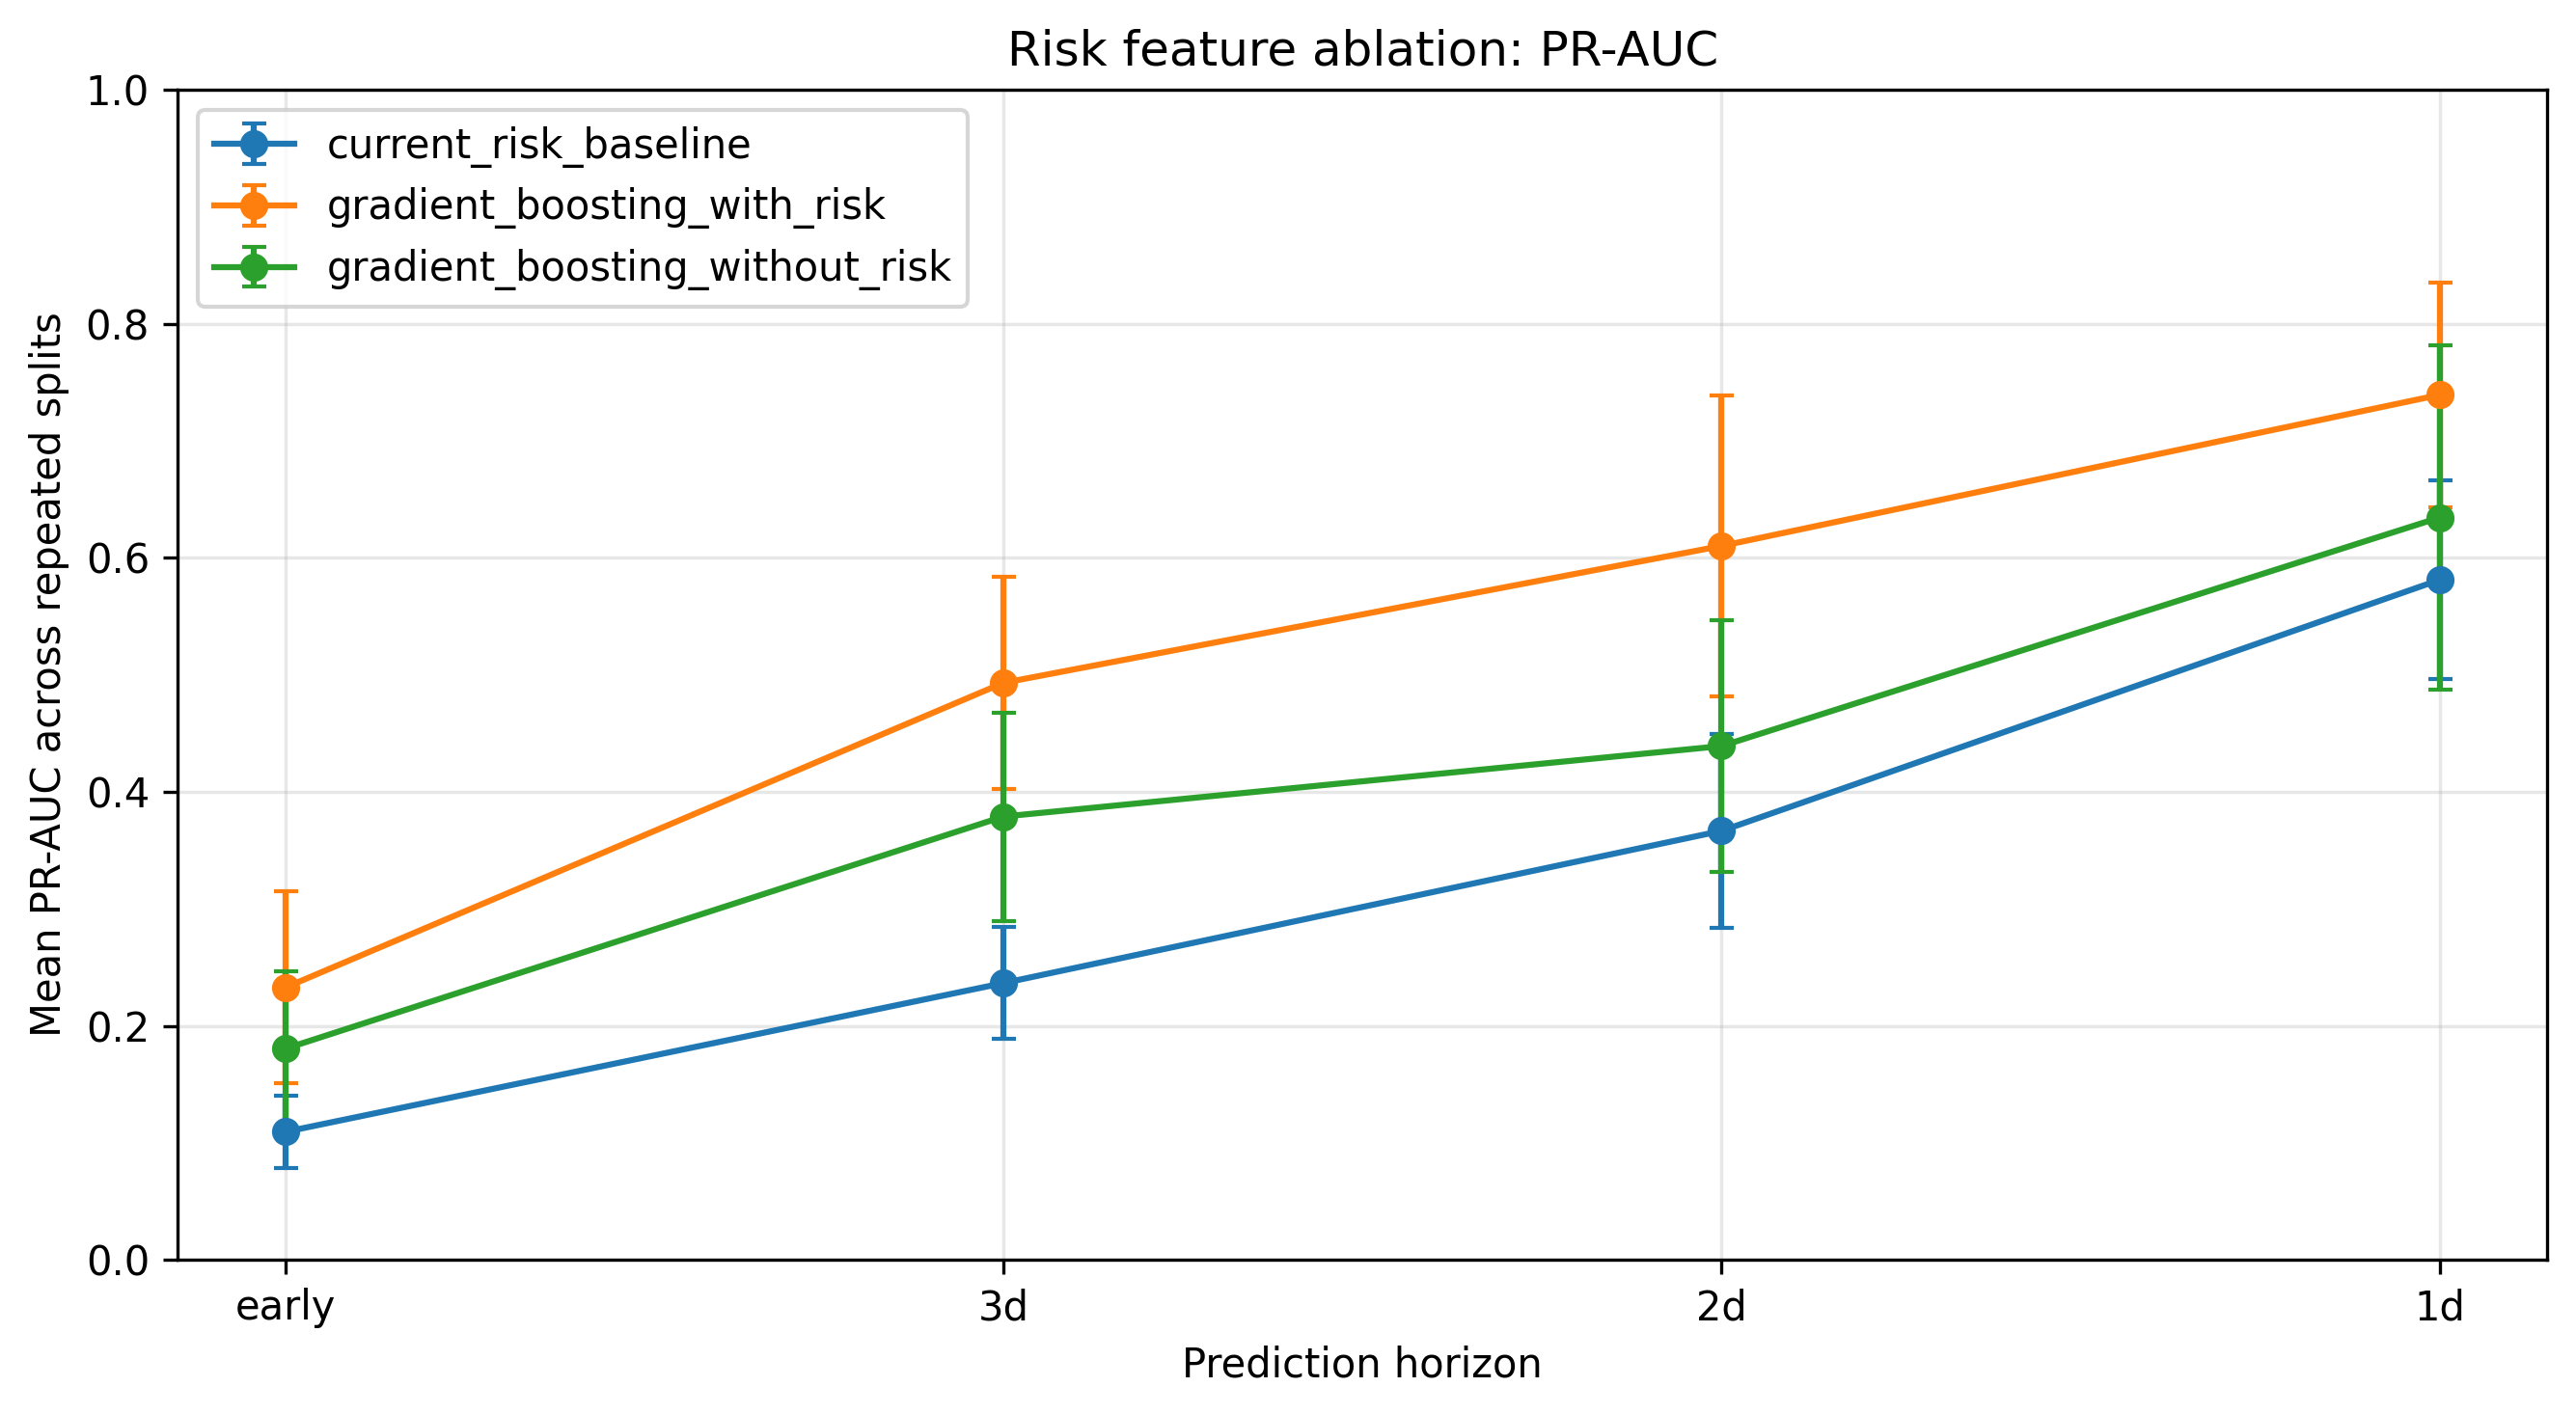
\includegraphics[width=\paperfigwidth]{risk_ablation_pr_auc.png}
    \caption{Risk feature ablation: PR-AUC.}
    \label{fig:risk-ablation-pr}
\end{figure}

\begin{figure}[!htbp]
    \centering
    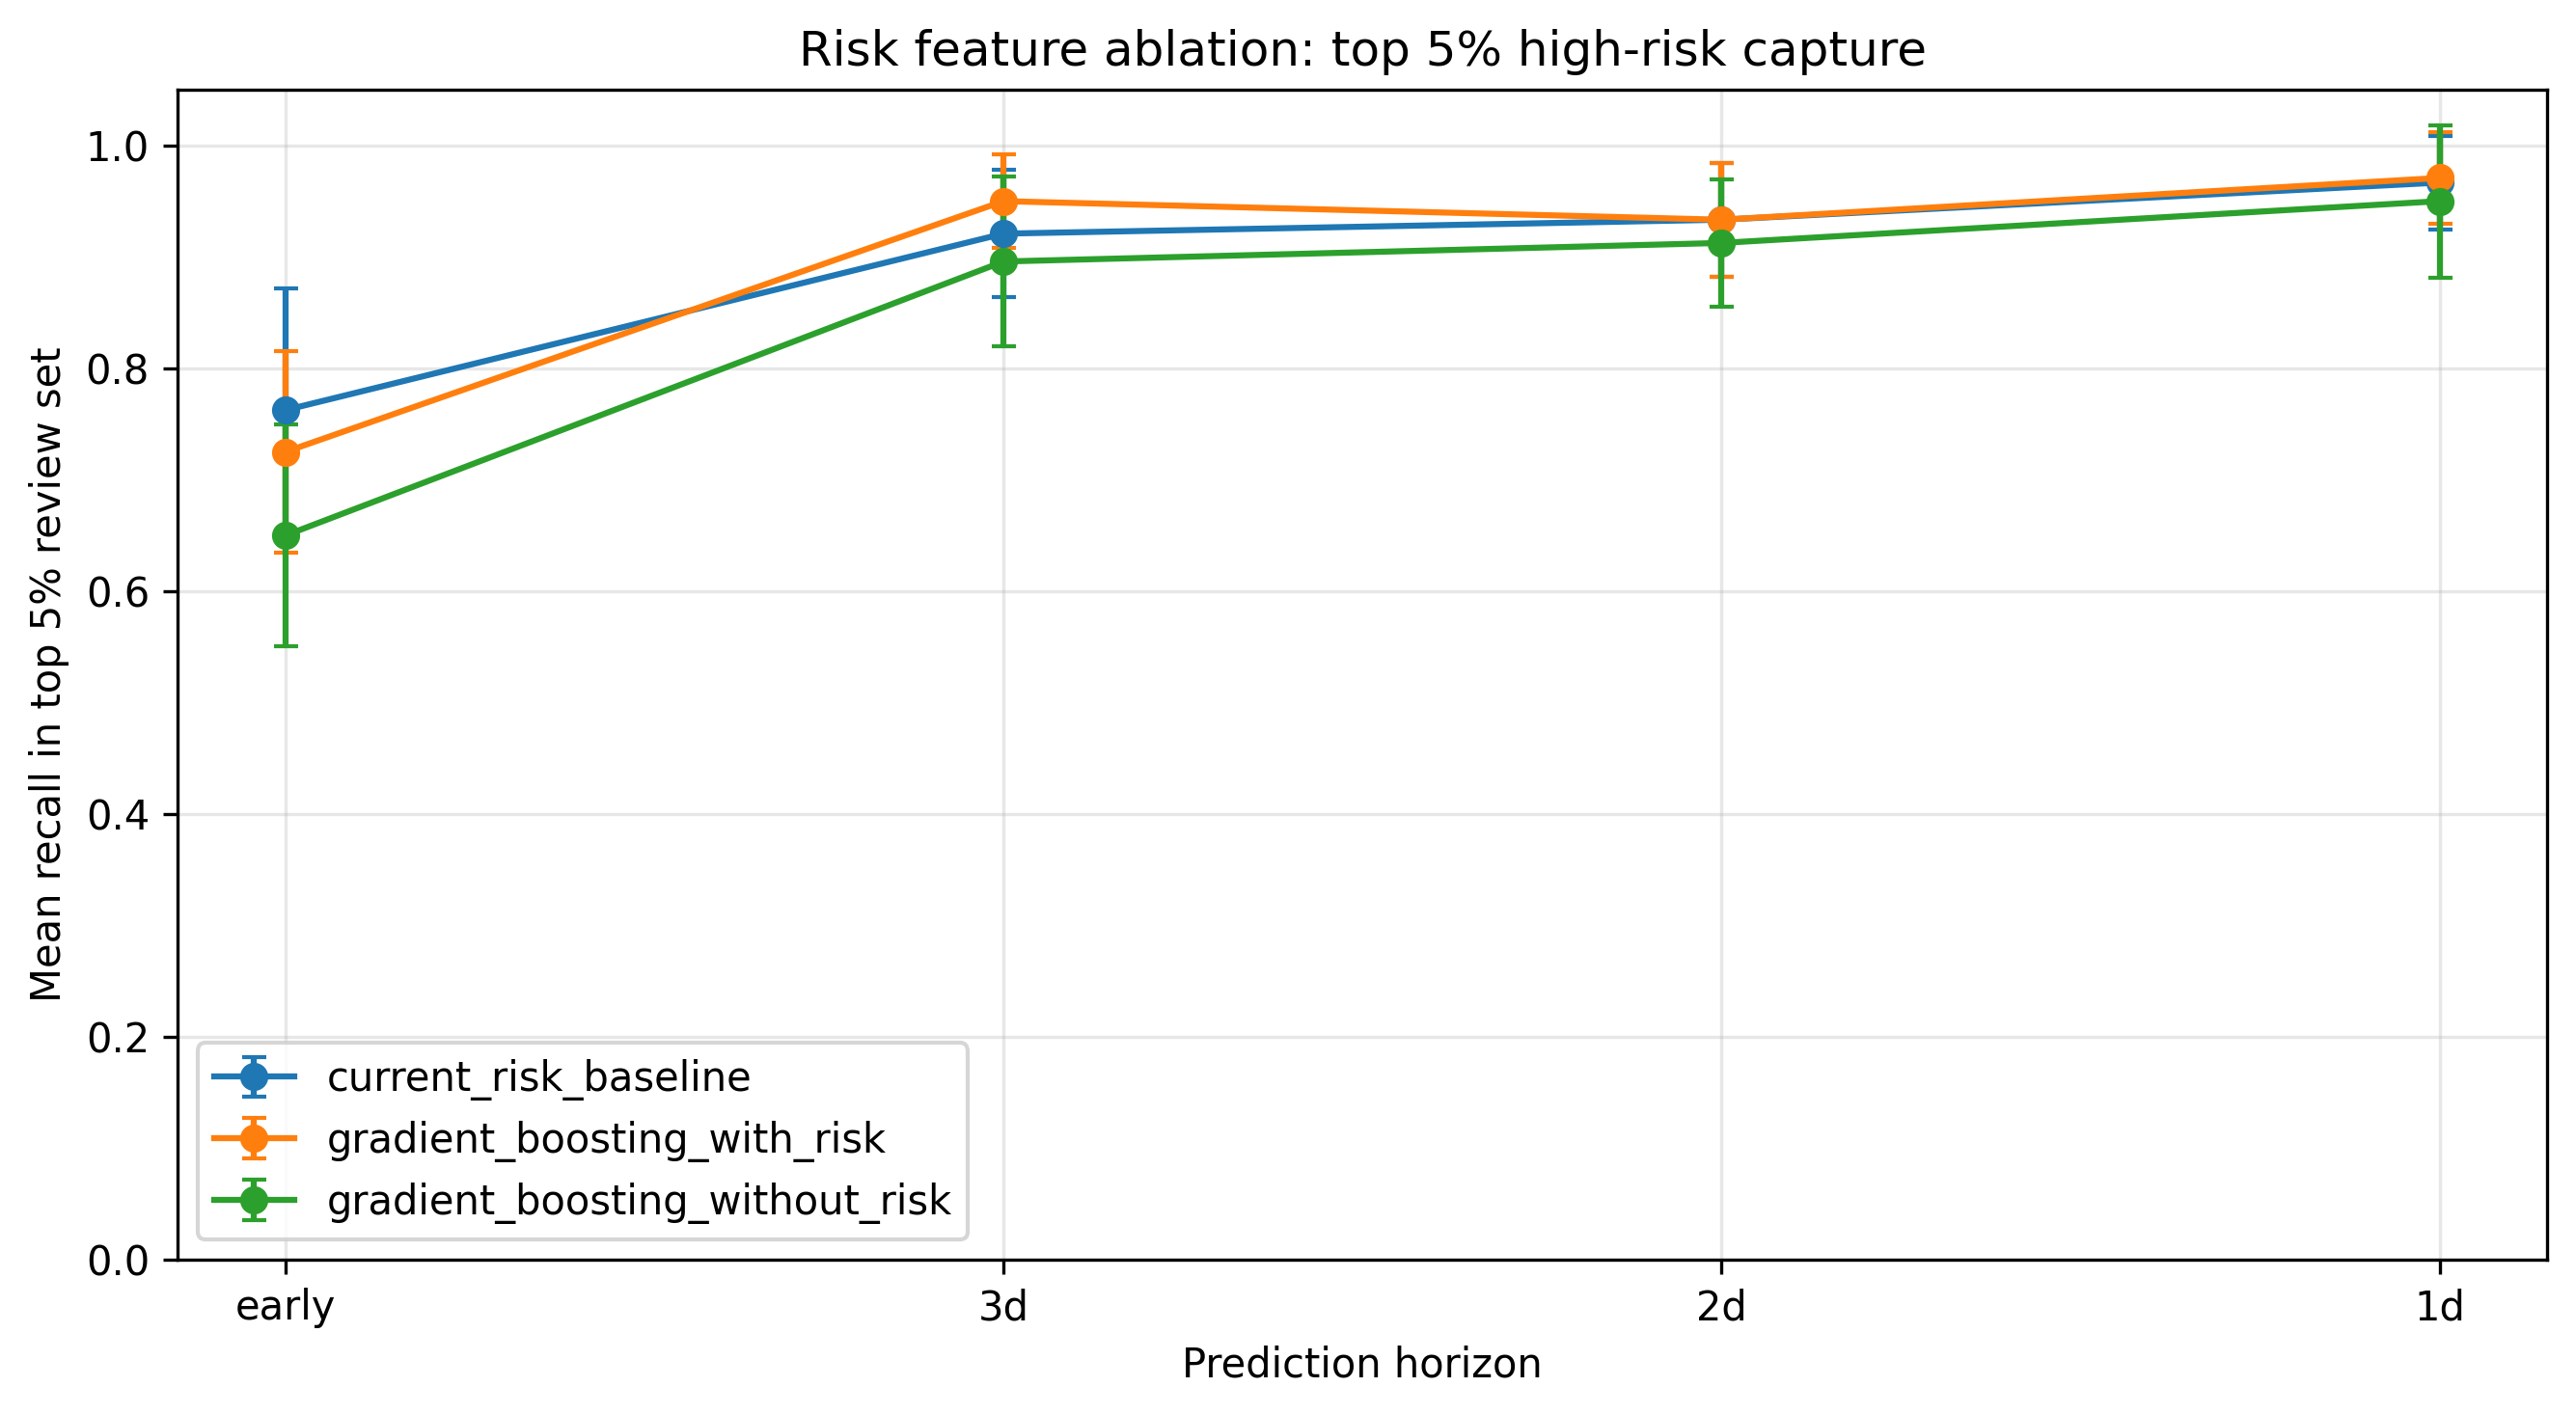
\includegraphics[width=\paperfigwidth]{risk_ablation_top5_recall.png}
    \caption{Risk feature ablation: top-5\% recall.}
    \label{fig:risk-ablation-top5}
\end{figure}

The ablation supports a nuanced interpretation. Current risk is an important signal: removing it consistently reduces gradient-boosting PR-AUC. However, the no-risk model still outperforms direct current-risk ranking in PR-AUC, suggesting that additional CDM/context features contain independent ranking signal. At the same time, direct current-risk ranking remains very competitive for top-K recall, especially near TCA. Therefore, the strongest claim is not that machine learning replaces current risk. The stronger and more defensible claim is that learned models can combine current risk with additional features to improve rare-event ranking, while current risk remains a central and operationally meaningful signal.

\FloatBarrier

\subsection{Repeated split robustness summary}

The repeated split analysis strengthens the evidence compared with a single held-out split. The positive class remains small, with about 12 high-risk events per test horizon, but the main qualitative results persist across 20 event-level splits: learned models improve PR-AUC over current-risk ranking at every horizon, top-K recall remains high for learned models, uncertainty escalation greatly outperforms random escalation, current-risk escalation remains a strong realistic comparator, and risk ablation shows that current risk is central but not the only predictive signal.

\section{Discussion}

The results suggest that calibrated and uncertainty-aware machine learning can support rare-event triage in satellite conjunction assessment.

The strongest use case is not replacing operational systems. Instead, BEACON is best understood as a decision-support framework for prioritizing which events deserve closer human review.

Five findings are especially important. First, the task is extremely imbalanced, with high-risk events representing less than 1\% of events. This makes accuracy an inappropriate primary metric. PR-AUC, top-K recall, calibration, uncertainty-aware escalation, risk ablation, and repeated split robustness are more meaningful. Second, learned models improve rare-event ranking over the current-risk baseline across repeated event-level splits. This matters because the current-risk baseline is a strong and realistic comparator. Third, uncertainty-based escalation captures most high-risk events by reviewing only a small fraction of the most uncertain predictions. This suggests that uncertainty estimates can help identify cases where automated prediction should defer to human judgment. Fourth, current-risk escalation remains extremely strong. This is not a weakness of BEACON. It is an important result: domain risk estimates already contain substantial signal, and learned uncertainty should be used to complement, not replace, domain-informed risk ranking. Fifth, the risk ablation shows that the current CDM risk feature is central to learned-model performance but does not fully explain the learned model's PR-AUC gains. The no-risk model still exceeds direct current-risk PR-AUC, while the with-risk model performs best. This supports an additive-feature interpretation rather than a replacement-of-risk interpretation.

\section{Limitations}

This project is a research prototype only. Key limitations include the small number of positive test events, reliance on public data only, lack of maneuver recommendation, lack of operational validation, Bayesian-inspired rather than fully Bayesian uncertainty for the strongest model, use of a research-defined high-risk threshold, and the possibility that learned feature relationships may not generalize to independent datasets.

Learned models include the current CDM risk feature in the main experiments, so results should be interpreted as improvement over direct current-risk ranking, not as risk-free prediction. Risk ablation reduces ambiguity about the current-risk feature, but it does not prove that learned feature relationships would generalize to other datasets. Events without pre-TCA observations require fallback handling and are tracked through diagnostics. The figures and metrics should be interpreted as preliminary evidence, not deployment-ready validation.

Because each test horizon contains only a small number of high-risk events, strong-looking recall results should still be interpreted cautiously. Repeating the evaluation across 20 event-level splits reduces single-split sensitivity, but it does not replace external validation on independent conjunction assessment data.

\section{Conclusion}

BEACON demonstrates a reproducible framework for evaluating trustworthy AI in satellite conjunction triage.

The project shows that rare-event ranking, calibration, uncertainty-aware escalation, risk-feature ablation, and repeated split robustness provide a more appropriate evaluation lens than accuracy alone. Learned models improve prioritization over direct current-risk ranking across 20 repeated event-level splits. The risk ablation shows that current risk is a central signal, but additional CDM/context features still contain ranking value. Bootstrap ensemble uncertainty identifies many high-risk events for human review and greatly outperforms random escalation, while remaining complementary to strong current-risk escalation.

Future work should add external validation, cost-sensitive metrics, operationally informed escalation policies, true Bayesian nonlinear models, richer uncertainty decomposition, and evaluation on additional conjunction datasets.

BEACON is not an operational collision-avoidance system. It is a research artifact showing how trustworthy machine learning methods can be evaluated for high-consequence space-domain decision support.

\section*{Artifact Availability}

Code, manuscript source, figures, tests, and reproduction scripts for the archived BEACON v0.2.2 research artifact are available through Zenodo at \href{https://doi.org/10.5281/zenodo.21209794}{doi:10.5281/zenodo.21209794} and through the associated GitHub repository. Raw ESA challenge data is not redistributed in the repository and must be obtained according to the original dataset provider's terms.

\bibliographystyle{plainnat}
\bibliography{references}

\end{document}
